\documentclass[a4 paper,12pt]{report}%eqno, fleqn, book,titlepage
\usepackage{amstext}
\usepackage{amsmath, amsfonts,latexsym, amscd, amsxtra, amssymb, amsbsy, amsgen, amsopn, fontenc, fontsmpl, amsthm}
\usepackage[mathscr]{eucal}
\usepackage{caption}
%\usepackage[tcvn]{vietnam}%dïng ®Ó §¸nh TiÕng ViÖt
\usepackage{graphicx}
\usepackage{fancyhdr}       		%T¹o tiªu ®Ò theo kiÓu míi
\let\up\MakeUppercase %vÝ dô: \up{viethoa}-->VIET HOA    
%---------******* §Þnh d¹ng trang giÊy*********--------------------------
\setlength{\textheight}{23cm} \setlength{\textwidth}{15.5cm}
\setlength{\oddsidemargin}{1cm} \setlength{\parindent}{1cm}
\setlength{\topmargin}{-0.3cm}
\renewcommand{\baselinestretch}{1.2}
\setlength{\parskip}{0cm}
\newcommand\brabar{\raisebox{-4.0pt}{\scalebox{.2}{
\textbf{(}}}\raisebox{-4.0pt}{{\_}}\raisebox{-4.0pt}{\scalebox{.2}{\textbf{)
}}}}

%----------
\usepackage{afterpage}
\newcommand\blankpage{%
	\null
	\thispagestyle{empty}%
	\addtocounter{page}{-1}%
	\newpage}
%%%%%%%%%%%%
\usepackage{mathptmx}
\usepackage{hyperref}
\hypersetup{
	colorlinks=false,
	pdfborder={0 0 0}
}
%\hypersetup{pdfborder=000, linkcolor=black}
\hyphenation{op-tical net-works semi-conduc-tor}
\def\Ml{\MakeLowercase}
%\def\Mr{\MakeUppercase}
\def\Mr{\uppercase}

% % % % % % % % % % % % % % % % % % % % % %
\usepackage{lineno}
\linenumbers
\usepackage{float}
%\usepackage{textcomp}
\usepackage{wasysym}%\permil 
\usepackage{graphicx,wrapfig,tikz}
\usepackage{caption}
\usepackage{subcaption}
%\usepackage{mathpazo}
\usepackage{amsmath,amsxtra,amssymb,latexsym,amscd,color,bm}
\usepackage[mathscr]{eucal}
\usepackage{epstopdf}
%\usepackage{biblatex}
% % % % % % % % %
\usepackage{array}
\usepackage{multirow}
\usepackage{cite}
\usepackage{ulem}
%-----------------------
\begin{document}
\title {}
\author{}
\pagestyle{plain}
\renewcommand\bibname{\centerline{\Large\up REFERENCES}}
\renewcommand\chaptername{\Large\up Chapter}
\renewcommand\contentsname{{\centerline{\Large\up TABLE OF CONTENT}}}
\makeatletter


%********************************************
\newpage 
\centerline{\LARGE {\up{\bf{technical note}}}}
\vspace{2cm}
\centerline{\Large {\up{\bf{combined sensitivities of T2K-II and NO$\nu$A}}}}
\centerline{\Large {\up{\bf{experiments to CP-violation}}}}
\centerline{\Large {\up{\bf{ in neutrino sector}}}}
\vspace{4cm}
\centerline{\LARGE {\up{\bf{tran van ngoc}}}}
\vspace{2cm}
\centerline{\LARGE {{\bf{Vietnam Neutrino Group}}}}
\centerline{\LARGE {{\bf{IFIRSE, Quy Nhon, VN}}}}
\tableofcontents
%\addcontentsline{toc}{section}{\up {\bf{table of content}}}

\newpage
\section{\Mr{Physics Motivation}}
%\centerline{\vntimeh{\huge begining}} \par
%\addcontentsline{toc}{section}{\up {\bf{Physics Motivation}}}
%\vspace{1cm}
\hspace{1cm}
In order to explain the solar neutrino anomaly \cite{Cleveland:1998nv} and atmospheric neutrino anomaly \cite{Hirata:1988uy}, neutrino oscillation phenomenon, in which one type of neutrino can change into another, has been proposed. In 1957, B. Pontecovo \cite{Pontecorvo:1957cp} firstly suggested a neutrino-antineutrino transition to explain these anomalies. The neutrino flavor oscillation was introduced later in 1962 by Z. Maki, M. Nakagawa and S. Sakata \cite{Maki:1962mu}. The neutrino oscillation phenomenon was observed  by Super-Kamiokande experiment~\cite{Fukuda:1998mi}, SNO experiment~\cite{Ahmad:2001an} and later conclusively confirmed by number of neutrino experiments with different detection techniques at different energy range and different baselines. Discovery of neutrino oscillation which indicates that neutrinos have mass and mix among states, matter a lot since this is the only experimental evidence for the incompleteness of the Standard Model of fundamental particles. 

Except for some anomalies, the up-to-date (anti-)neutrino data from various experiments can be well described by a $3\times$ 3 unitary mixing matrix, so-called PMNS matrix. This unitary matrix, as discussed more details in the next section, are parameterized by three mixing angles ($\theta_{12}$, $\theta_{13}$ and $\theta_{23}$) and one single Dirac phase $\delta_{\text{CP}}$\footnote{If neutrino is Majorana particle, there are two phases added into the PMNS matrix. However the oscillation amplitudes are not sensitive to these two phases.} which represents CP violation in the lepton sector.  The three mixing angles are determined to be non-zero \cite{Patrignani:2016xqp} and this allows neutrino experiments to make measurement on the CP violation in the lepton sector, which is one of the most central objective in the present and at near future of neutrino physics. Besides these four parameters, the oscillation probabilities depend on the mass-squared differences among the mass eigenstate, neutrino energy and the distance neutrino travels. At the current landscape of neutrino oscillation physics, two scales of mass-squared differences are determined. However their mass ordering is still unknown and also one of the most important question need to be addressed in the future.


 T2K and NOvA are two among the world leading neutrino experiments in searching the CP violation in the lepton sector. The combined sensitivity of these two experiments was performed and shows that this sensitivity can be up to 2$\sigma$ or higher if the true value $\delta_{CP}$ is about $-\pi/2$ \cite{Abe:2014tzr}. We are revising this analysis with three main updates including (i) possible T2K run extension up to 2026, so-called T2K-II (ii) improvement in selection performance and systematic uncertainties in both experiment and (iii) the ultimate precision on mixing angle $\theta_{13}$ can be achieved by the reactor measurements. The first twos are crucial since the measurement is dominated by the statistical errors. The thirds one is needed to break down the $\delta_{CP}-\theta_{13}$ degeneracy with accelerator-based long baseline experiment.These combined critical factors enhances capability to search CP violation to unprecedented level of sensitivity.
 

The paper is organised as follows, the PMNS formalism of neutrino oscillation is  introduced with an intense focus on how CP violation can be measured. T2K(-II) and NOvA experiments are overviewed and their inputs for this analysis are presented in section \ref{sec:t2knova}. The  outcomes of combined sensitivity between the T2K-II and NOvA experiment with constraint from reactor are presented in section \ref{sec:results}.\par 
%%%%%%%%%%%%%%%%%%%%%%%%%%%%%%%%%%%
 \section{\Mr{Neutrino oscillation framework}}\label{sec:oscframework}
%%%%%%%%%%%%%%%%%%%%%%%%%%%%%%%%%%%

In three-flavor neutrino oscillation framework, the flavor definitive eigenstates are related to the mass definitive eigenstates by a $3 \times 3$ unitary PMNS matrix, shown in Eq.~\ref{eq:1}, \par
\begin{equation}\label{eq:1}
\left(\begin{array}{ccc}\nu_e\\ \nu_\mu\\ \nu_\tau\end{array}\right)=U_{\text{PMNS}}\left(\begin{array}{ccc}\nu_1\\ \nu_2\\ \nu_3\end{array}\right)=\left(\begin{array}{ccc}U_{e1}& U_{e2} & U_{e3}\\U_{\mu 1} & U_{\mu 2} & U_{\mu 3}\\U_{\tau 1}& U_{\tau 2}& U_{\tau 3}\end{array}\right)\left(\begin{array}{ccc}\nu_1\\ \nu_2\\ \nu_3\end{array}\right).
\end{equation}
The unitarity of PMNS matrix $UU^{\dagger} = I$ yields nine independent parameters. If the PMNS matrix were real, it could be described by three rotation angles $\theta_{12}, \theta_{13}$ and $\theta_{23}$ via orthogonal rotation matrix R
 \begin{equation}\label{38}
 R= \left(\begin{array}{ccc} 1& 0 & 0 \\ 0 & c_{23} & s_{23}\\ 0& - s_{23}& c_{23}\end{array}\right) \left(\begin{array}{ccc} c_{13}& 0 & s_{13}\\ 0 & 1&0 \\-s_{13}& 0 & c_{13} \end{array}\right) \left(\begin{array}{ccc}c_{12} & s_{12} & 0\\ -s_{12} & c_{12} & 0\\ 0 & 0 & 1\end{array}\right)
\end{equation} 
where $s_{ij} = \sin{\theta_{ij}}$ and $c_{ij} = \cos\theta_{ij}$. Since PMNS matrix is unitary and not real, it must contain six more additional degrees of freedom in term of complex phase $e^{i\delta}$. Five among these six phases can be absorbed into the definition of the particles and leaves only one single phase $\delta$. This can be seen as follow.\par
The charged currents for leptonic weak interaction
$$-i\frac{g_W}{\sqrt{2}}(\bar{e}, \bar{\mu}, \bar{\tau})\gamma^{\mu}\frac{1}{2}(1-\gamma^5)\left(\begin{array}{ccc}U_{e1}& U_{e2} & U_{e3}\\U_{\mu 1} & U_{\mu 2} & U_{\mu 3}\\U_{\tau 1}& U_{\tau 2}& U_{\tau 3}\end{array}\right)\left(\begin{array}{ccc}\nu_1\\ \nu_2\\ \nu_3\end{array}\right)$$
The four-vector currents are unchanged by transformation
\begin{equation}\label{transform}
l_\alpha \rightarrow l_\alpha e^{i\theta_\alpha}, \quad \nu_k \rightarrow \nu_k e^{i\theta_k}\quad \text{and} \quad U_{\alpha k} \rightarrow U_{\alpha k} e^{i(\theta_\alpha - \theta_k)}
\end{equation}
where $l_\alpha$ is the charged lepton of the type $\alpha = e, \mu, \tau$. Since the phases are arbitrary, all other phases can be defined in term of $\theta_e$: 
$$\theta_k = \theta_e + \theta'_k$$
The transformation (\ref{transform}) therefore becomes
$$l_\alpha \rightarrow l_\alpha e^{i(\theta_e + \theta'_\alpha)}, \quad \nu_k \rightarrow \nu_k e^{i(\theta_e + \theta'_k)}\quad \text{and} \quad U_{\alpha k} \rightarrow U_{\alpha k} e^{i(\theta'_\alpha - \theta'_k)}$$
For electron $\theta_e = \theta_e + \theta'_e \quad \Rightarrow \theta'_e = 0$. It is can be seen now that only five phases are independent and can be absorbed into the particle definitions. The PMNS matrix thus can be parameterized by three mixing angles ($\theta_{12}, \theta_{13}, \theta_{23}$) and a single  Dirac phase $\delta_{CP}$, expressed in Eq.~\ref{eq:2}.
 \begin{eqnarray}\label{eq:2}\nonumber
U_{PMNS} &=& \left(\begin{array}{ccc}U_{e1}& U_{e2} & U_{e3}\\U_{\mu 1} & U_{\mu 2} & U_{\mu 3}\\U_{\tau 1}& U_{\tau 2}& U_{\tau 3}\end{array}\right)\\  \nonumber 
&=& \left(\begin{array}{ccc} 1& 0 & 0 \\ 0 & c_{23} & s_{23}\\ 0& - s_{23}& c_{23}\end{array}\right) \left(\begin{array}{ccc} c_{13}& 0 & s_{13}e^{-i\delta}\\ 0 & 1&0 \\-s_{13}e^{i\delta}& 0 & c_{13} \end{array}\right) \left(\begin{array}{ccc}c_{12} & s_{12} & 0\\ -s_{12} & c_{12} & 0\\ 0 & 0 & 1\end{array}\right) \\ 
&=&  \left(\begin{array}{ccc}c_{12}c_{13}& s_{12}c_{13} & s_{13}e^{-i\delta}\\ -s_{12}c_{23} - c_{12}s_{23}s_{13}e^{i\delta} & c_{12}c_{23} - s_{12}s_{23}s_{13}e^{i\delta}& s_{23}c_{13}\\ s_{12}s_{23}-c_{12}c_{23}s_{13}e^{i\delta}& -c_{12}s_{23}-s_{12}c_{23}s_{13}e^{i\delta} & c_{23}c_{13}\end{array}\right)
\end{eqnarray}
where $s_{ij} = \sin{\theta_{ij}}$, $c_{ij} = \cos\theta_{ij}$ and $\delta_{CP}$ Dirac phase represents the CP violation in lepton sector \footnote{If neutrino is Majorana particle, the mixing matrix includes two additional phases which do not appear in the expression of oscillation probabilities.}.
As mentioned before, CP is violated if $U^*_{\alpha i}U_{\beta i}U_{\alpha_j}U^*_{\beta_j}$ contains an imaginary component. Therefore, $\delta$ is also called the CP-violating phase $\delta_{CP}$.  

The oscillation probability from muon neutrino to electron neutrino is
   \begin{eqnarray}\label{10}
P(\nu_\mu \rightarrow \nu_e) &=& |\langle \nu_e |\Psi(\vec x, t)\rangle|^2 = c_ec_e^*\nonumber \\
&=& |U^*_{\mu 1}U_{e1}e^{-i\phi_1}+U^*_{\mu 2}U_{e2}e^{-i\phi_2}+U^*_{\mu3}U_{e3}e^{-i\phi_3}|^2
   \end{eqnarray} \par

In compact form
   \begin{eqnarray}\label{11}
P(\nu_\alpha \rightarrow \nu_\beta) = |\sum_iU^*_{\alpha i}U_{\beta i}e^{-i\phi_i}|^2
   \end{eqnarray} \par
If $\phi_1 = \phi_2 = \phi_3 (\approx \frac{m^2}{2E})$, from unitary condition we have $P(\nu_\alpha \rightarrow \nu_\beta) = \delta_{\alpha\beta}$. This means that the oscillations occur if the neutrinos have mass and the masses are not the same.

Using the identity properties of complex number:
\begin{equation}\label{12}
|z_1+z_2+z_3|^2 = |z_1|^2+|z_2|^2+|z_3|^2+2Re[z_1z_2^*+z_1z_3^*+z_2z_3^*]
\end{equation}\par
Then equation (\ref{10}) becomes
   \begin{eqnarray}\label{13}
 P(\nu_\mu \rightarrow \nu_e) &=& |U^*_{\mu 1}U_{e1}e^{-i\phi_1}+U^*_{\mu 2}U_{e2}e^{-i\phi_2}+U^*_{\mu3}U_{e3}e^{-i\phi_3}|^2\nonumber \\
&=&  |U^*_{\mu 1}U_{e1}|^2 +|U^*_{\mu 2}U_{e2}|^2+|U^*_{\mu3}U_{e3}|^2 \nonumber\\
&+& 2Re[U^*_{\mu 1}U_{e1}U_{\mu_2}U^*_{e2}e^{i(\phi_2-\phi_1)}] \nonumber\\
&+& 2Re[U^*_{\mu 1}U_{e1}U_{\mu_3}U^*_{e3}e^{i(\phi_3-\phi_1)}] \nonumber\\
&+& 2Re[U^*_{\mu 2}U_{e2}U_{\mu_3}U^*_{e3}e^{i(\phi_3-\phi_2)}]
   \end{eqnarray} \par
In compact form
   \begin{eqnarray}\label{14}
P(\nu_\alpha \rightarrow \nu_\beta) = \sum_i|U^*_{\alpha i}U_{\beta i}|^2 + 2\sum_{j>i} Re[U^*_{\alpha i}U_{\beta i}U_{\alpha j}U^*_{\beta_j} e^{i(\phi_j-\phi_i)}]
   \end{eqnarray} \par

From the unitary condition we derive
   \begin{eqnarray}\label{15}
& &|U^*_{\mu 1}U_{e1}+U^*_{\mu 2}U_{e2}+U^*_{\mu3}U_{e3}|^2 = 0\nonumber\\
&\Rightarrow& |U^*_{\mu 1}U_{e1}|^2 +|U^*_{\mu 2}U_{e2}|^2+|U^*_{\mu3}U_{e3}|^2 \nonumber\\
&+& 2Re[U^*_{\mu 1}U_{e1}U_{\mu_2}U^*_{e2}+ U^*_{\mu 1}U_{e1}U_{\mu_3}U^*_{e3}+ U^*_{\mu 2}U_{e2}U_{\mu_3}U^*_{e3}]\nonumber\\
&=& 0
   \end{eqnarray} \par

In compact form 
   \begin{eqnarray}\label{16}
 \sum_i|U^*_{\alpha i}U_{\beta i}|^2 + 2\sum_{j>i} Re[U^*_{\alpha i}U_{\beta i}U_{\alpha j}U^*_{\beta_j}] =\delta_{\alpha\beta}
   \end{eqnarray} \par
It is followed from (\ref{13}) and (\ref{15}):
   \begin{eqnarray}\label{17}
 P(\nu_\mu \rightarrow \nu_e)
&=& 2Re\left[U^*_{\mu 1}U_{e1}U_{\mu_2}U^*_{e2} \left(e^{i(\phi_2-\phi_1)}-1\right)\right] \nonumber\\
&+& 2Re\left[U^*_{\mu 1}U_{e1}U_{\mu_3}U^*_{e3} \left(e^{i(\phi_3-\phi_1)}-1\right)\right] \nonumber\\
&+& 2Re\left[U^*_{\mu 2}U_{e2}U_{\mu_3}U^*_{e3} \left(e^{i(\phi_3-\phi_2)}-1\right)\right]
   \end{eqnarray} \par

In compact form 
   \begin{eqnarray}\label{18}
P(\nu_\alpha \rightarrow \nu_\beta) =\delta_{\alpha\beta}+ 2\sum_{j>i} Re[U^*_{\alpha i}U_{\beta i}U_{\alpha j}U^*_{\beta_j}(e^{i(\phi_j-\phi_i)})-1)] 
   \end{eqnarray} \par
We have
   \begin{eqnarray}\label{19}
& &Re[U^*_{\alpha i}U_{\beta i}U_{\alpha j}U^*_{\beta_j}(e^{i(\phi_j-\phi_i)})-1)]\nonumber\\
&=& Re[U^*_{\alpha i}U_{\beta i}U_{\alpha j}U^*_{\beta_j}(\cos(\phi_j-\phi_i)-1 +i\sin(\phi_j-\phi_i))]\nonumber\\
&=&Re\left\{(Re[U^*_{\alpha i}U_{\beta i}U_{\alpha j}U^*_{\beta_j}]+ i Im[U^*_{\alpha i}U_{\beta i}U_{\alpha j}U^*_{\beta_j}])(-2\sin^2(\frac{\phi_j-\phi_i}{2})+i\sin(\phi_j-\phi_i))\right\} \nonumber\\
&=&-2Re[U^*_{\alpha i}U_{\beta i}U_{\alpha j}U^*_{\beta_j}]\sin^2(\frac{\phi_j-\phi_i}{2})- Im[U^*_{\alpha i}U_{\beta i}U_{\alpha j}U^*_{\beta_j}]\sin(\phi_j-\phi_i) 
   \end{eqnarray} \par

From (\ref{19}), we can write the oscillation pobability in a normal form
   \begin{eqnarray}\label{20}
 &&P(\nu_\mu \rightarrow \nu_e) = \nonumber\\
&-& 4Re\left[U^*_{\mu 1}U_{e1}U_{\mu_2}U^*_{e2}\right]\sin^2(\frac{\phi_2-\phi_1}{2})-2Im\left[U^*_{\mu 1}U_{e1}U_{\mu_2}U^*_{e2}\right]\sin(\phi_2-\phi_1) \nonumber\\
&-& 4Re\left[U^*_{\mu 1}U_{e1}U_{\mu_3}U^*_{e3}\right]\sin^2(\frac{\phi_3-\phi_1}{2})-2Im\left[U^*_{\mu 1}U_{e1}U_{\mu_3}U^*_{e3}\right]\sin(\phi_3-\phi_1) \nonumber\\
&-& 4Re\left[U^*_{\mu 2}U_{e2}U_{\mu_3}U^*_{e3}\right]\sin^2(\frac{\phi_3-\phi_2}{2})-2Im\left[U^*_{\mu 2}U_{e2}U_{\mu_3}U^*_{e3}\right]\sin(\phi_3-\phi_2)
   \end{eqnarray} \par
In compact form
   \begin{eqnarray}\label{21}
 P(\nu_\alpha \rightarrow \nu_\beta) =\delta_{\alpha\beta}&-& 4\sum_{j>i}Re\left[U^*_{\alpha i}U_{\beta i}U_{\alpha_j}U^*_{\beta_j}\right]\sin^2(\frac{\phi_j-\phi_i}{2}) \nonumber\\
&-& 2\sum_{j>i}Im\left[U^*_{\alpha i}U_{\beta i}U_{\alpha_j}U^*_{\beta_j}\right]\sin(\phi_j-\phi_i)
   \end{eqnarray} \par


If the neutrino interacts at a time T at a distance L along its direction of flight, the difference in phase of the three mass eigenstates are written as
$$\phi_j-\phi_i =p_j.x_j - p_i.x_i = (E_j-E_i)T-(p_j-p_i)L$$ \par

With assuming that $p_j=p_i = p$ for neutrinos of the same source, then
   \begin{eqnarray}\label{22}
\phi_j-\phi_i& =&(E_j-E_i)T \approx \left[p_j(1+\frac{m_j^2}{2p_j^2}) - p_i(1+\frac{m_i^2}{2p^2_i})\right]T\nonumber\\
&=&\frac{m_j^2-m_i^2}{2p}T = \frac{\Delta m^2_{ji}L}{2E}
   \end{eqnarray} \par
In the above calculation, we used the approximation $T \approx L$ and $p \approx E$ for $v_\nu \approx c $ and $m_\nu \ll E_\nu$

We finally get the most common form of the oscillation probability:
   \begin{eqnarray}\label{23}
 P(\nu_\alpha \rightarrow \nu_\beta) =\delta_{\alpha\beta}&-& 4\sum_{j>i}Re\left[U^*_{\alpha i}U_{\beta i}U_{\alpha_j}U^*_{\beta_j}\right]\sin^2(\frac{\Delta m^2_{ji}}{4E}L) \nonumber\\
&-& 2\sum_{j>i}Im\left[U^*_{\alpha i}U_{\beta i}U_{\alpha_j}U^*_{\beta_j}\right]\sin(\frac{\Delta m^2_{ji}}{2E}L)
   \end{eqnarray} \par

\textcolor{red}{The probability for a $\alpha$-flavour neutrino with energy $E$ to change to $\beta$-flavour after traveling a distance of $L$ can be calculated as follows 
 \begin{align}\label{eq:2add}
 P(\nu_\alpha \rightarrow \nu_\beta) =& \delta_{\alpha \beta}-4\sum_{i>j}\Re\left[U^*_{\alpha i}U_{\beta i}U_{\alpha_j}U^*_{\beta_j}\right]\sin^2\left(\frac{\Delta m^2_{ij}}{4E}L\right) + 2\sum_{i>j}\Im\left[U^*_{\alpha i}U_{\beta i}U_{\alpha_j}U^*_{\beta_j}\right]\sin\left(\frac{\Delta m^2_{ij}}{2E}L\right),
 \end{align}
where $\Delta m^2_{ij} = m^2_{i} - m^2_{j}$. For antineutrinos, the oscillation probabilities can be obtained by replace the mixing matrix elements with their complex conjugate.}\par 
\textcolor{blue}{Equation (\ref{eq:2add}) is completely the same as eq. (\ref{23})}.\par 
For antineutrinos, we just take the complex conjugate of the product matrix and get
   \begin{eqnarray}\label{24}
 P(\bar\nu_\alpha \rightarrow \bar\nu_\beta) =\delta_{\alpha\beta}&-& 4\sum_{j>i}Re\left[U^*_{\alpha i}U_{\beta i}U_{\alpha_j}U^*_{\beta_j}\right]\sin^2(\frac{\Delta m^2_{ji}}{4E}L) \nonumber\\
&+& 2\sum_{j>i}Im\left[U^*_{\alpha i}U_{\beta i}U_{\alpha_j}U^*_{\beta_j}\right]\sin(\frac{\Delta m^2_{ji}}{2E}L)
   \end{eqnarray} \par
The probabilities (\ref{23}) and (\ref{24}) are called \textit{transition probabilities}, and the \textit{survival probability} for a flavor is
 
   \begin{equation}\label{25}
 P(\nu_\alpha \rightarrow \nu_\alpha) = P(\bar\nu_\alpha \rightarrow \bar\nu_\alpha) =1- 4\sum_{j>i}|U_{\alpha i}|^2|U_{\alpha_j}|^2\sin^2(\frac{\Delta m^2_{ji}}{4E}L)
   \end{equation} \par

By using the natural unit conversion for $1eV^{-1}\text{of length} = 1.97 \times 10^{-7}m$, we can practically express the phase in (\ref{23}), (\ref{24}) and (\ref{25}) as
   \begin{eqnarray}\label{26}
&& \frac{\Delta m^2_{ji}[eV^2] L[eV]}{4E[eV]} = \frac{\Delta m^2_{ji}[eV^2] L[m]}{4\times 1.97\times 10^{-7}E[eV]} \nonumber\\
&&=1.269 \frac{\Delta m^2_{ji}[eV^2] L[m]}{E[MeV]} = 1.269 \frac{\Delta m^2_{ji}[eV^2] L[km]}{E[GeV]}
   \end{eqnarray}



From (\ref{23}) and (\ref{24}), the difference between the neutrino and antineutrino oscillation probability indicates CP violation in neutrino sector
   \begin{eqnarray}\label{27}
 \mathcal{A}_{\text{CP}} &=&P(\nu_\alpha \rightarrow \nu_\beta)-P(\bar\nu_\alpha \rightarrow \bar\nu_\beta) \nonumber\\
&=& 4\sum_{j>i}Im\left[U^*_{\alpha i}U_{\beta i}U_{\alpha_j}U^*_{\beta_j}\right]\sin(\frac{\Delta m^2_{ij}}{2E}L)
   \end{eqnarray} \par
If CP is violated, $U^*_{\alpha i}U_{\beta i}U_{\alpha_j}U^*_{\beta_j}$ has to contain an imaginary component. \par
For $\alpha = \mu$ and $\beta = e$, then
   \begin{eqnarray}\label{28} 
\mathcal{A}_{\text{CP}} &=&P(\nu_\mu \rightarrow \nu_e)-P(\bar\nu_\mu \rightarrow \bar\nu_e) \nonumber\\
&=& 4\sum_{j>i}Im\left[U^*_{\mu i}U_{e i}U_{\mu_j}U^*_{e_j}\right]\sin(\frac{\Delta m^2_{ij}}{2E}L) \\ 
&=& 4Im\left[U^*_{\mu 1}U_{e 1}U_{\mu_2}U^*_{e_2}\right]\sin(\frac{\Delta m^2_{12}}{2E}L) \nonumber \\
&+& 4Im\left[U^*_{\mu 1}U_{e 1}U_{\mu_3}U^*_{e_3}\right]\sin(\frac{\Delta m^2_{13}}{2E}L) \nonumber \\
&+& 4Im\left[U^*_{\mu 2}U_{e 2}U_{\mu_3}U^*_{e_3}\right]\sin(\frac{\Delta m^2_{23}}{2E}L)  
  \end{eqnarray} \par
From the unitary condition we have
   \begin{eqnarray}\label{30} 
U_{\mu 1}U^*_{e 1} + U_{\mu_2}U^*_{e_2} + U_{\mu 3}U^*_{e3} = 0  
  \end{eqnarray} \par
Multiply two sides of the equation (\ref{30}) with $U^*_{\mu 1} U_{e1}$ and $U^*_{\mu 2} U_{e2}$ respectively and then add them up, we have
   \begin{eqnarray}\label{31} 
& &U^*_{\mu 1} U_{e1}U_{\mu 1}U^*_{e 1} + U^*_{\mu 1} U_{e1}U_{\mu_2}U^*_{e_2} + U^*_{\mu 1} U_{e1}U_{\mu 3}U^*_{e3}\nonumber \\
 &+ &U^*_{\mu 2} U_{e2}U_{\mu 1}U^*_{e 1} + U^*_{\mu 2} U_{e2}U_{\mu_2}U^*_{e_2} + U^*_{\mu 2} U_{e2}U_{\mu 3}U^*_{e3} = 0 \nonumber\\
&\Leftrightarrow& 0 = |U_{\mu 1}|^2|U_{e1}|^2 + |U_{\mu 2}|^2 |U_{e2}|^2 \nonumber \\ 
&+& Re[U^*_{\mu 1} U_{e1}U_{\mu_2}U^*_{e_2}] + Re[U^*_{\mu 2} U_{e2}U_{\mu 1}U^*_{e 1}] + Re[U^*_{\mu 1} U_{e1}U_{\mu 3}U^*_{e3}] + Re[U^*_{\mu 2} U_{e2}U_{\mu 3}U^*_{e3}] \nonumber \\
&+& i\left\{Im[U^*_{\mu 1} U_{e1}U_{\mu_2}U^*_{e_2}] + Im[U^*_{\mu 2} U_{e2}U_{\mu 1}U^*_{e 1}] + Im[U^*_{\mu 1} U_{e1}U_{\mu 3}U^*_{e3}] + Im[U^*_{\mu 2} U_{e2}U_{\mu 3}U^*_{e3}] \right\} \nonumber \\
&\Rightarrow& Im[U^*_{\mu 1} U_{e1}U_{\mu_2}U^*_{e_2}] + Im[U^*_{\mu 2} U_{e2}U_{\mu 1}U^*_{e 1}] + Im[U^*_{\mu 1} U_{e1}U_{\mu 3}U^*_{e3}] + Im[U^*_{\mu 2} U_{e2}U_{\mu 3}U^*_{e3}] = 0 \nonumber \\
  \end{eqnarray} \par
Note that $$[U^*_{\mu 1} U_{e1}U_{\mu_2}U^*_{e_2}]^*= U^*_{\mu 2} U_{e2}U_{\mu 1}U^*_{e 1} \Rightarrow Im[U^*_{\mu 1} U_{e1}U_{\mu_2}U^*_{e_2}]=-Im [U^*_{\mu 2} U_{e2}U_{\mu 1}U^*_{e 1}]$$
Therefore, from (\ref{31}) we get
\begin{equation}\label{32}
Im[U^*_{\mu 1} U_{e1}U_{\mu 3}U^*_{e3}] = - Im[U^*_{\mu 2} U_{e2}U_{\mu 3}U^*_{e3}]
\end{equation}\par

Multiply two sides of the equation (\ref{30}) with $U^*_{\mu 1} U_{e1}$ and $U^*_{\mu 3} U_{e3}$ respectively and then add them up, we have
   \begin{eqnarray}\label{33} 
& &U^*_{\mu 1} U_{e1}U_{\mu 1}U^*_{e 1} + U^*_{\mu 1} U_{e1}U_{\mu_2}U^*_{e_2} + U^*_{\mu 1} U_{e1}U_{\mu 3}U^*_{e3}\nonumber \\
 &+ &U^*_{\mu 3} U_{e3}U_{\mu 1}U^*_{e 1} + U^*_{\mu 3} U_{e3}U_{\mu_2}U^*_{e_2} + U^*_{\mu 3} U_{e3}U_{\mu 3}U^*_{e3} = 0 \nonumber\\
&\Leftrightarrow& 0 = |U_{\mu 1}|^2|U_{e1}|^2 + |U_{\mu 3}|^2 |U_{e3}|^2 \nonumber \\ 
&+& Re[U^*_{\mu 1} U_{e1}U_{\mu_3}U^*_{e_3}] + Re[U^*_{\mu 3} U_{e3}U_{\mu 1}U^*_{e 1}] + Re[U^*_{\mu 1} U_{e1}U_{\mu 2}U^*_{e2}] + Re[U^*_{\mu 3} U_{e3}U_{\mu 2}U^*_{e2}] \nonumber \\
&+& i\left\{Im[U^*_{\mu 1} U_{e1}U_{\mu_3}U^*_{e_3}] + Im[U^*_{\mu 3} U_{e3}U_{\mu 1}U^*_{e 1}] + Im[U^*_{\mu 1} U_{e1}U_{\mu 2}U^*_{e2}] + Im[U^*_{\mu 3} U_{e3}U_{\mu 2}U^*_{e2}] \right\} \nonumber \\
&\Rightarrow& Im[U^*_{\mu 1} U_{e1}U_{\mu_3}U^*_{e_3}] + Im[U^*_{\mu 3} U_{e3}U_{\mu 1}U^*_{e 1}] + Im[U^*_{\mu 1} U_{e1}U_{\mu 2}U^*_{e2}] + Im[U^*_{\mu 3} U_{e3}U_{\mu 2}U^*_{e2}] = 0 \nonumber \\
  \end{eqnarray} \par
Note that $$[U^*_{\mu 1} U_{e1}U_{\mu_3}U^*_{e_3}]^*= U^*_{\mu 3} U_{e3}U_{\mu 1}U^*_{e 1} \Rightarrow Im[U^*_{\mu 1} U_{e1}U_{\mu_3}U^*_{e_3}]= - Im[U^*_{\mu 3} U_{e3}U_{\mu 1}U^*_{e 1}]$$ 
 and
$$[U^*_{\mu 3} U_{e3}U_{\mu 2}U^*_{e2}]^* =  U^*_{\mu 2} U_{e2}U_{\mu 3}U^*_{e3} \Rightarrow Im[U^*_{\mu 3} U_{e3}U_{\mu 2}U^*_{e2}] =  - [U^*_{\mu 2} U_{e2}U_{\mu 3}U^*_{e3}]$$
Therefore, from (\ref{33}) we get
\begin{equation}\label{34}
Im[U^*_{\mu 1} U_{e1}U_{\mu 2}U^*_{e2}] = Im[U^*_{\mu 2} U_{e2}U_{\mu 3}U^*_{e3}]
\end{equation}\par

By using (\ref{32}) and (\ref{34}), we can rewrite (29) as
   \begin{eqnarray}\label{35} 
\mathcal{A}_{\text{CP}} &=&P(\nu_\mu \rightarrow \nu_e)-P(\bar\nu_\mu \rightarrow \bar\nu_e) \nonumber\\
&=& 4Im\left[U^*_{\mu 1}U_{e 1}U_{\mu_3}U^*_{e_3}\right] \left( \sin\Delta_{13} - \sin\Delta_{12} - \sin\Delta_{23}\right)
  \end{eqnarray} \par
Where $\Delta_{13} = \frac{\Delta m^2_{13}}{2E}L$, $ \Delta_{12}=\frac{\Delta m^2_{12}}{2E}L$ and $ \Delta_{23} =\frac{\Delta m^2_{23}}{2E}L = \Delta_{13} - \Delta_{23}$ \par
By a simple trigonometry calculation, we have
   \begin{eqnarray}\label{36} 
\sin\Delta_{13} - \sin\Delta_{12} - \sin(\Delta_{13} - \Delta_{12}) &=& - 4 \sin\frac{\Delta_{12}}{2}\sin\frac{\Delta_{13}}{2}\sin\frac{\Delta_{23}}{2}\nonumber \\
&=& 4 \sin\frac{\Delta_{21}}{2}\sin\frac{\Delta_{31}}{2}\sin\frac{\Delta_{32}}{2}\nonumber 
  \end{eqnarray} \par
Then we can rewrite (\ref{35}) as
   \begin{eqnarray}\label{37} 
&&\mathcal{A}_{\text{CP}} =P(\nu_\mu \rightarrow \nu_e)-P(\bar\nu_\mu \rightarrow \bar\nu_e) \nonumber\\
&& = 16Im\left[U^*_{\mu 1}U_{e 1}U_{\mu_3}U^*_{e_3}\right] \left(  \sin\frac{\Delta_{21}}{2}\sin\frac{\Delta_{31}}{2}\sin\frac{\Delta_{32}}{2}\right)\nonumber \\
&& = 16Im\left[U^*_{\mu 1}U_{e 1}U_{\mu_3}U^*_{e_3}\right]   \sin\left(\frac{\Delta m^2_{21}L}{4E}\right)\sin\left(\frac{\Delta m^2_{31}L}{4E}\right)\sin\left(\frac{\Delta m^2_{32}L}{4E}\right)
  \end{eqnarray} \par

The general form in term of oscillation parameters can be obtained as shown in Eq.~\ref{eq:3}. \textcolor{red}{The coefficients in the denominator should be 4 instead of 2!
%%there is no reason why dCP should appear along with theta_13. It can go with theta_12 or theta23.
\noindent 
   \begin{align}\label{eq:3}
% \text{CP violation term} &=&P(\nu_\alpha \rightarrow \nu_\beta)-P(\bar\nu_\alpha \rightarrow \bar\nu_\beta) \nonumber\\
\mathcal{A}_{\text{CP}}=&P(\nu_\alpha \rightarrow \nu_\beta)-P(\bar\nu_\alpha \rightarrow \bar\nu_\beta) 
= 4\sum_{j>i}\Im\left[U^*_{\alpha i}U_{\beta i}U_{\alpha_j}U^*_{\beta_j}\right]\sin\left(\frac{\Delta m^2_{ji}}{2E}L\right), \nonumber \\
=&\pm 2 \delta_{\alpha \beta} \cos \theta_{13} \sin 2\theta_{12} \sin 2\theta_{23} \sin 2\theta_{13} \sin \delta_{CP} \sin \frac{\Delta m^2_{21}L}{4E}  \sin \frac{\Delta m^2_{32} L}{4E}  \sin \frac{\Delta m^2_{13} L }{4E}
   \end{align}}
in which $\{\alpha, \beta\} = \{e, \mu, \tau\}$; $\{i, j\} = \{1, 2, 3\}$, $j > i$ and $\Delta m^2_{ji} = m^2_j - m^2_i$; the positive (negative) sign is applied based on (anti-) cyclic permutation of ordered flavor ($e,\mu,\tau$). Apparently CP violation can be measured via the neutrino oscillation phenomenon if only three mixing angles are non-zero. The up-to-date neutrino data shows that Nature supports this scenario and it opens the door to search CP violation in the lepton sector with neutrino oscillation measurements. This CP violation source might be a promising explanation for the matter asymmetry in the Universe. \par

%%%%%%%%Should mention that nu_mu to nu_e is the main channel
%%%%%%%nu_mu to nu_mu can be help to beak some degeneracy
%\red{are two leading accelerator-based long baseline neutrino experiment in the world}.

In practical, CP violation can be measured by comparing the rate of electron neutrinos appearance from muon neutrinos, $P(\nu_\mu \rightarrow \nu_e)$, with its of electron antineutrinos appearance from muon anti-neutrinos, $P(\overline{\nu}_\mu \rightarrow \overline{\nu}_e)$ in accelerator-based experiments or comparing the first with electron antineutrino disappearance in the reactor-based experiments\footnote{Accelerator-based measurements leads to an intrinsic $\delta_{CP}-\theta_{13}$ degeneracy while reactor-based measurement can precisely measure $\theta_{13}$. Their combined information thus can provide constraint on $\delta_{CP}$.}

$*$ \textbf{Evolution of neutrino flavors in matter}\par
The relation between mass eigenstates and flavor eigenstates
   \begin{eqnarray}\nonumber
|\nu_\alpha\left.\right> = \sum_kU^*_{\alpha k}|\nu_k\left. \right> 
   \end{eqnarray} 
 The total Hamiltonian in matter is
   \begin{eqnarray}\nonumber
H = H_0 + H_1
   \end{eqnarray} 
Where 
   \begin{eqnarray}\nonumber
H_0|\nu_k\left.\right> &=& E_k|\nu_k\left.\right>; \quad \text{with}\quad E_k = \sqrt{\vec{p_k}^2+m_k^2}\approx p_k + \frac{m^2_k}{2p_k}\\ \nonumber
H_1|\nu_\alpha\left.\right> &=& V_\alpha|\nu_\alpha\left.\right>
   \end{eqnarray} 
The Schrodinger equation for neutrino in matter is
   \begin{eqnarray}\nonumber
i\frac{d}{dt}|\nu_\alpha(t)\left.\right> &=& H|\nu_\alpha(t)\left.\right> \\ \nonumber
 &=& (H_0+ H_1)|\nu_\alpha(t)\left.\right> \\ \nonumber
 &=& (E_k + V_\alpha)|\nu_\alpha(t)\left.\right> \\ \nonumber
&=&  \left[\left(p_k + \frac{m^2_k}{2p_k}\right) + V_\alpha\right]|\nu_\alpha(t)\left.\right> 
   \end{eqnarray} 
For $v \approx c$ (means $t \approx x$) we have $p_k \approx E$. We can see that $E + V_{NC}$ is the same for all neutrinos. They generate a phase common to all flavors and will cancel out in transition. Hence we can ignore them here for simplicity. So we rewrite the above equation as
   \begin{eqnarray}\nonumber
i\frac{d}{dt}|\nu_\alpha(t)\left.\right> = \left( \frac{m^2_k}{2E}+V_{CC}\delta_{\alpha e}\right)|\nu_\alpha(t)\left.\right> 
   \end{eqnarray} 
Or in explicit form
\begin{eqnarray} \label{56}
i\frac{d}{dt}\left(\begin{array}{ccc}\nu_e\\ \nu_\mu\\ \nu_\tau\end{array}\right)= \left[\frac{1}{2E}U\left(\begin{array}{ccc}m^2_1&0&0\\0&m^2_2&0\\ 0&0& m^2_3\end{array}\right)U^{\dagger}+\left(\begin{array}{ccc}V_{CC}&0&0\\0&0&0\\ 0&0&0\end{array}\right)\right]\left(\begin{array}{ccc}\nu_e\\ \nu_\mu\\ \nu_\tau\end{array}\right)
\end{eqnarray}
Where $U$ is an unitary matrix.\par

$*$ \textbf{Complete oscillation probability in matter}\par
Since $v \approx c$ so $x \approx ct = t$ for $c =1$. We can rewrite the Schrodinger equation in matter as
$$i\frac{d\nu}{dx} = H\nu$$
Where
 \begin{eqnarray}\label{62}\nonumber
H &=& H_0 + H_1\\ \nonumber
 &=&  \frac{1}{2E}U\left(\begin{array}{ccc} 0&0&0\\0&0&0\\ 0&0& \Delta m^2_{31}\end{array}\right)U^\dagger + 
 \frac{1}{2E}\left[U\left(\begin{array}{ccc} 0&0&0\\0&\Delta m^2_{21}&0\\ 0&0&0\end{array} \right)U^\dagger + \left(\begin{array}{ccc} a&0&0\\0&0&0\\ 0&0&0 \end{array}\right)\right]
\end{eqnarray} 
and $a = 2EV_{CC} = 2\sqrt{2}G_FEN_e$.\par
Since $\Delta m^2_{21}$ and $ a \ll \Delta m^2_{31}$, we can treat $H_1$ as a pertubation.\par
The Schrodinger equation has a solution of Dyson series form 
\begin{equation}\label{63}
\nu(x) =S(x)\nu(0)
\end{equation}
With $$S(x) \equiv Te^{\int^x_0H(s)ds}$$
T is the symbol of time ordering. The oscillation probability at distance $L$ then can be calculate through $S(x)$
\begin{equation}\label{64}
P(\nu_{\alpha} \rightarrow \nu_{\beta}) = |S_{\beta\alpha}(L)|^2
\end{equation}
We can calculate the pertubation to the first order in $a$ and $\Delta m^2_{21}$. We have
$$S_0(x) = e^{-iH_0x}$$
and
$$S_1(x) = e^{-iH_0x}(-i)\int^x_0dsH_1(s) =  e^{-iH_0x}(-i)\int^x_0dse^{iH_0s}H_1e^{-iH_0s}$$
We now calculate $S_0(x)$ and $S_1(x)$ as the following\par
 \begin{eqnarray}\nonumber
(S_0(x))_{\beta\alpha} &=& \left[ Ue^{-i\frac{x}{2E}diag(0,0,\Delta m^2_{31})}U^\dagger\right]_{\beta\alpha}\\ \nonumber
&=& \sum_{i,j}\left[ U_{\beta i}\left(e^{-i\frac{x}{2E}diag(0,0,\Delta m^2_{31})}\right)_{ij}U^*_{\alpha j}\right]
\end{eqnarray} 
Note that 
$$e^{-i\frac{x}{2E}diag(0,0,\Delta m^2_{31})} = \left(\begin{array}{ccc} 1&0&0\\0&1&0\\ 0&0&e^{-i\frac{\Delta m^2_{31}x}{2E}}\end{array}\right)$$
Hence
 \begin{eqnarray}\nonumber
(S_0(x))_{\beta\alpha} &=&U_{\beta 1}U^*_{\alpha 1}.1 + U_{\beta 1}U^*_{\alpha 2}.0+U_{\beta 1}U^*_{\alpha 3}.0\\ \nonumber
&&+ U_{\beta 2}U^*_{\alpha 1}.0 + U_{\beta 2}U^*_{\alpha 2}.1+U_{\beta 2}U^*_{\alpha 3}.0\\ \nonumber
&&+ U_{\beta 3}U^*_{\alpha 1}.0 + U_{\beta 3}U^*_{\alpha 2}.0+U_{\beta 2}U^*_{\alpha 3}.e^{-i\frac{\Delta m^2_{31}x}{2E}}\\ \nonumber
&=&U_{\beta 1}U^*_{\alpha 1} + U_{\beta 2}U^*_{\alpha 2}+U_{\beta 3}U^*_{\alpha 3}.e^{-i\frac{\Delta m^2_{31}x}{2E}}
\end{eqnarray}
By using $U_{\beta 1}U^*_{\alpha 1} + U_{\beta 2}U^*_{\alpha 2}+U_{\beta 3}U^*_{\alpha 3} = \delta_{\alpha\beta}$ \quad$\Rightarrow$ 
\begin{equation}\label{65}
(S_0(x))_{\beta\alpha}=\delta_{\alpha\beta} + U_{\beta 3}U^*_{\alpha 3}\left(e^{-i\frac{\Delta m^2_{31}x}{2E}} - 1\right)
\end{equation}
Similarity for calculating $(S_1(x))_{\beta\alpha}$. We have
 \begin{eqnarray}\nonumber
(S_1(x))_{\beta\alpha} &=& \left(e^{-iH_0x}(-i)\int^x_0dse^{iH_0s}H_1e^{-iH_0 s}\right)_{\beta\alpha}\\ \nonumber
&=& -i \int^x_0ds\left(e^{-iH_0(x-s)}H_1e^{-iH_0s}\right)_{\beta\alpha}\\ \nonumber
&=& -i  \int^x_0ds\left(Ue^{-i\frac{x-s}{2E}diag(0,0,\Delta m^2_{31})}U^\dagger H_1Ue^{-i\frac{s}{2E}diag(0,0,\Delta m^2_{31})}U^\dagger\right)_{\beta\alpha}\\ \nonumber
&=& -i  \int^x_0ds\sum_{i,j',i',j}\left[U_{\beta i}\left(e^{-i\frac{x-s}{2E}diag(0,0,\Delta m^2_{31})}\right)_{ij'}U^*_{\gamma j'} (H_1)_{\gamma \sigma}U_{\sigma i'}\left(e^{-i\frac{s}{2E}diag(0,0,\Delta m^2_{31})}\right)_{i'j}U^*_{\beta j}\right]
\end{eqnarray}
Since $\left(e^{-i\frac{x-s}{2E}diag(0,0,\Delta m^2_{31})}\right)_{ij'} = 0$ for $j' \not= i$\par
and $\left(e^{-i\frac{s}{2E}diag(0,0,\Delta m^2_{31})}\right)_{i'j} = 0$ for $i' \not= j$ \quad $\Rightarrow$
 \begin{eqnarray}\nonumber
(S_1(x))_{\beta\alpha} &=& -i  \int^x_0ds\sum_{i,j}\left[U_{\beta i}\left(e^{-i\frac{x-s}{2E}diag(0,0,\Delta m^2_{31})}\right)_{ii}U^*_{\gamma i} (H_1)_{\gamma \sigma}U_{\sigma j}\left(e^{-i\frac{s}{2E}diag(0,0,\Delta m^2_{31})}\right)_{jj}U^*_{\beta j}\right]\\ 
&=&-i \sum_{i,j}U_{\beta i}U^*_{\gamma i} (H_1)_{\gamma \sigma}U_{\sigma j}U^*_{\beta j} \int^x_0ds\left(e^{-i\frac{\Delta m^2_{31}}{2E}[(x-s)\delta_{i3}+ s\delta_{j3}}\right)
\end{eqnarray}
Let 
$$X_{ij} =U_{\beta i}U^*_{\gamma i} (H_1)_{\gamma \sigma}U_{\sigma j}U^*_{\beta j}$$ 
and 
$$Y_{ij} = \int^x_0ds\left(e^{-i\frac{\Delta m^2_{31}}{2E}[(x-s)\delta_{i3}+ s\delta_{j3}}\right)= \int^x_0ds\left(e^{-i\frac{\Delta m^2_{31}x}{2E}\delta_{i3}}.e^{-i\frac{\Delta m^2_{31}s}{2E}(\delta_{j3} -\delta_{i3}}\right)$$
We first calculate the $X_{ij}$ term\par
We see that $$U^*_{\gamma i} (H_1)_{\gamma \sigma}U_{\sigma j} = \frac{1}{2E}[U^*_{\gamma i} (V_{12})_{\gamma \sigma}U_{\sigma j}+U^*_{\gamma i} (V_a)_{\gamma \sigma}U_{\sigma j}]$$
Since $(V_{12})_{22} = \Delta m^2_{21}$ and $(V_{12})_{\gamma \sigma} = 0$ for $\gamma \not= 2$ or $\sigma \not= 2$ then
$$\frac{1}{2E}U^*_{\gamma i} (V_{12})_{\gamma \sigma}U_{\sigma j} = \frac{\Delta m^2_{21}}{2E}\delta_{2i}\delta_{2j}$$
Since $(V_{a})_{11} =a$ and $(V_{a})_{\gamma \sigma} = 0$ for $\gamma \not= 1$ or $\sigma \not= 1$ then
$$\frac{1}{2E}U^*_{\gamma i} (V_{a})_{\gamma \sigma}U_{\sigma j} = \frac{a}{2E}U^*_{1i}U_{1j}$$ 
Therefore
$$U^*_{\gamma i} (H_1)_{\gamma \sigma}U_{\sigma j} = \frac{\Delta m^2_{21}}{2E}\delta_{2i}\delta_{2j}+  \frac{a}{2E}U^*_{1i}U_{1j}$$
and
 \begin{eqnarray}\label{66}\nonumber
X_{ij} &=&U_{\beta i}U^*_{\gamma i} (H_1)_{\gamma \sigma}U_{\sigma j}U^*_{\beta j}\\ \nonumber
&=&U_{\beta i}\left[\frac{\Delta m^2_{21}}{2E}\delta_{2i}\delta_{2j}+  \frac{a}{2E}U^*_{1i}U_{1j}\right] U^*_{\alpha j}\\ 
&=&\frac{\Delta m^2_{21}}{2E}U_{\beta i} U^*_{\alpha j}\delta_{2i}\delta_{2j}+  \frac{a}{2E}U_{\beta i}U^*_{1i}U_{1j} U^*_{\alpha j}
\end{eqnarray}
and the $Y_{ij}$ integral is
 \begin{eqnarray}\nonumber
Y_{11} &=&Y_{12} = Y_{21} = Y_{22} = x\\ \nonumber 
Y_{13} &=&Y_{23} = Y_{31} = Y_{32} = \left(-i\frac{\Delta m^2_{31}}{2E}\right)^{-1}\left(e^{-i\frac{\Delta m^2_{31}x}{2E}}-1\right)\\ \nonumber 
Y_{33} &=&xe^{-i\frac{\Delta m^2_{31}x}{2E}}
\end{eqnarray}
In general
 \begin{eqnarray}\label{67}
Y_{ij} &=& (1-\delta_{i3})(1-\delta_{j3})x + \delta_{i3}\delta_{j3}xe^{-i\frac{\Delta m^2_{31}x}{2E}} \\ \nonumber
&&+[(1-\delta_{i3})\delta_{j3} + \delta_{i3}(1-\delta_{j3})]\left(-i\frac{\Delta m^2_{31}}{2E}\right)^{-1}\left(e^{-i\frac{\Delta m^2_{31}x}{2E}}-1\right)
\end{eqnarray}
Insert (\ref{67}) and (\ref{66}) into (\ref{65}) we get
 \begin{eqnarray}\nonumber
(S_1(x))_{\beta\alpha} &=& -i\frac{ax}{2E}e^{-i\frac{\Delta m^2_{31}x}{2E}}U_{\beta 3}U^*_{\alpha 3}|U_{13}|^2\\ \nonumber
&&-ix\left[\frac{\Delta m^2_{21}}{2E}U_{\beta 2}U^*_{\alpha 2}+ \frac{a}{2E}(U_{\beta 1}U^*_{11}U_{11}U^*_{\alpha 1}+U_{\beta 1}U^*_{11}U_{12}U^*_{\alpha 2}\right.\\ \nonumber
&&\left.+U_{\beta 2}U^*_{12}U_{11}U^*_{\alpha 1} +U_{\beta 2}U^*_{12}U_{12}U^*_{\alpha 2})\right]\\ \nonumber
&&-i\left(-i\frac{\Delta m^2_{31}}{2E}\right)^{-1}\left(e^{-i\frac{\Delta m^2_{31}x}{2E}}-1\right)\frac{a}{2E}(U_{\beta 1}U^*_{11}U_{13}U^*_{\alpha 3}+U_{\beta 2}U^*_{12}U_{13}U^*_{\alpha 3} \\ \nonumber
&&+U_{\beta 3}U^*_{13}U_{11}U^*_{\alpha 1} +U_{\beta 3}U^*_{13}U_{12}U^*_{\alpha 2})
\end{eqnarray}
Note that $\sum^2_{k=1}U^*_{\alpha k}U_{1k} = \delta_{\alpha 1}-U^*_{\alpha 3}U_{13}$. We now can calculate the factors that are relevant to matrix elements as the following
 \begin{eqnarray}\nonumber
&&U_{\beta 1}U^*_{11}U_{11}U^*_{\alpha 1}+U_{\beta 1}U^*_{11}U_{12}U^*_{\alpha 2}+U_{\beta 2}U^*_{12}U_{11}U^*_{\alpha 1}+U_{\beta 2}U^*_{12}U_{12}U^*_{\alpha 2}\\ \nonumber
&=&(U_{\beta 1}U^*_{11}+U_{\beta 2}U^*_{12})(U_{11}U^*_{\alpha 1}+U_{12}U^*_{\alpha 2})\\ \nonumber
&=&(\delta_{\beta 1}-U_{\beta 3}U^*_{13})(\delta_{\alpha 1}-U_{13}U^*_{\alpha 3})\\ \nonumber
&=& \delta_{\alpha 1}\delta_{\beta 1}-\delta_{\alpha 1}U_{\beta 3}U^*_{13}-\delta_{\beta 1}U_{13}U^*_{\alpha 3}+U_{\beta 3}U^*_{\alpha 3}|U_{13}|^2\\ \nonumber
&=&\delta_{\alpha 1}\delta_{\beta 1}+U_{\beta 3}U^*_{\alpha 3}(|U_{13}|^2-\delta_{\alpha 1}-\delta_{\beta 1})
\end{eqnarray}
 \begin{eqnarray}\nonumber
 &&U_{\beta 1}U^*_{11}U_{13}U^*_{\alpha 3}+U_{\beta 2}U^*_{12}U_{13}U^*_{\alpha 3}+U_{\beta 3}U^*_{13}U_{11}U^*_{\alpha 1}+U_{\beta 3}U^*_{13}U_{12}U^*_{\alpha 2}\\ \nonumber
&=&U_{13}U^*_{\alpha 3}(\delta_{\beta 1}-U_{\beta 3}U^*_{13})+ U_{\beta 3}U^*_{13}(\delta_{\alpha 1} -U_{13}U^*_{\alpha 3})\\ \nonumber
&=& \delta_{\alpha 1}U_{\beta 3}U^*_{13}+\delta_{\beta 1}U_{13}U^*_{\alpha 3} -2U_{\beta 3}U^*_{\alpha 3}|U_{13}|^2\\ \nonumber
&=&U_{\beta 3}U^*_{\alpha 3}(\delta_{\alpha 1}+\delta_{\beta 1}-2|U_{13}|^2)
\end{eqnarray}
Therefore
 \begin{eqnarray}\label{68} \nonumber
(S_1(x))_{\beta\alpha} &=& -i\frac{ax}{2E}e^{-i\frac{\Delta m^2_{31}x}{2E}}U_{\beta 3}U^*_{\alpha 3}|U_{13}|^2\\ \nonumber
&&-i\frac{x}{2E}\left[\Delta m^2_{21}U_{\beta 2}U^*_{\alpha 2}+a(\delta_{\alpha 1}\delta_{\beta 1}+U_{\beta 3}U^*_{\alpha 3}(|U_{13}|^2 -\delta_{\alpha 1}-\delta_{\beta 1}))\right]\\
&&-\frac{a}{\Delta m^2_{31}}\left(e^{-i\frac{\Delta m^2_{31}x}{2E}}-1\right)(2|U_{13}|^2 -\delta_{\alpha 1}-\delta_{\beta 1})U_{\beta 3}U^*_{\alpha 3}
\end{eqnarray}
From (\ref{68}) and (\ref{65}) and note that $\sin X/2 = \frac{e^{iX/2} - e^{-iX/2}}{2i}$ with $X = \frac{\Delta m^2_{31}}{2E}$ we get
 \begin{eqnarray} \nonumber
(S(x))_{\beta\alpha} &=&(S_0(x))_{\beta\alpha} +(S_1(x))_{\beta\alpha}\\ \nonumber
 &=&\delta_{\alpha\beta} + U_{\beta 3}U^*_{\alpha 3}\left(e^{-i\frac{\Delta m^2_{31}x}{2E}} - 1\right) -\frac{a}{\Delta m^2_{31}}\left(e^{-i\frac{\Delta m^2_{31}x}{2E}}-1\right)(2|U_{13}|^2 -\delta_{\alpha 1}-\delta_{\beta 1})U_{\beta 3}U^*_{\alpha 3} \\ \nonumber
&& -i\frac{ax}{2E}e^{-i\frac{\Delta m^2_{31}x}{2E}}U_{\beta 3}U^*_{\alpha 3}|U_{13}|^2 +\left(i\frac{ax}{2E}U_{\beta 3}U^*_{\alpha 3}|U_{13}|^2 -i\frac{ax}{2E}U_{\beta 3}U^*_{\alpha 3}|U_{13}|^2\right)\\ \nonumber
&&-i\frac{\Delta m^2_{31}x}{2E}\left[\frac{\Delta m^2_{21}}{\Delta m^2_{31}}U_{\beta 2}U^*_{\alpha 2}+\frac{a}{\Delta m^2_{31}}(\delta_{\alpha 1}\delta_{\beta 1}+U_{\beta 3}U^*_{\alpha 3}(|U_{13}|^2 -\delta_{\alpha 1}-\delta_{\beta 1}))\right]
\end{eqnarray}

By rearranging the common terms the above equation becomes
 \begin{eqnarray}\label{69} \nonumber
(S(x))_{\beta\alpha} &=&\delta_{\alpha\beta} -i2e^{-i\Delta_{31}}\sin\Delta_{31}U_{\beta 3}U^*_{\alpha 3}\left[(1-C)-\frac{iax}{2E}|U_{13}|^2\right]\\  \nonumber
&&-i2\Delta_{31}\left[\epsilon U_{\beta 2}U^*_{\alpha 2}+\frac{a}{\Delta m^2_{31}}\delta_{\alpha 1}\delta_{\beta 1}+CU_{\beta 3}U^*_{\alpha 3}\right] \\
&=& \delta_{\alpha\beta} + A + B
\end{eqnarray}
Where $\Delta_{31} = \frac{\Delta m^2_{31}x}{4E}$; $\epsilon = \frac{\Delta m^2_{21}}{\Delta m^2_{31}}$ and $C = \frac{a}{\Delta m^2_{31}}(2|U_{13}|^2-\delta_{\alpha 1}-\delta_{\beta 1})$\par

The oscillation probability now can be calculated 
 \begin{eqnarray}\label{70} \nonumber
P(\nu_\alpha \rightarrow \nu_\beta) &=& |(S(x))_{\beta\alpha}|^2 \\ 
&=& \delta_{\alpha\beta}(1 + A + A^* + B + B^*) + AA^* + BB^* + A^*B + AB^*
\end{eqnarray}\par
$\bullet$ The tearm which is relevant to $\delta_{\alpha\beta}$
 \begin{eqnarray} \nonumber
&&\delta_{\alpha\beta}(1 + A + A^* + B + B^*)\\ \nonumber
&=&\delta_{\alpha\beta}\left\{ 1 - i2e^{-i\Delta_{31}}\sin\Delta_{31}U_{\beta 3}U^*_{\alpha 3}\left[(1-C)-\frac{iax}{2E}|U_{13}|^2\right]\right. \\  \nonumber
&&  + i2e^{i\Delta_{31}}\sin\Delta_{31}U^*_{\beta 3}U_{\alpha 3}\left[(1-C)+\frac{iax}{2E}|U_{13}|^2\right] \\ \nonumber
&&-i2\Delta_{31}\left[\epsilon U_{\beta 2}U^*_{\alpha 2}+\frac{a}{\Delta m^2_{31}}\delta_{\alpha 1}\delta_{\beta 1}+CU_{\beta 3}U^*_{\alpha 3}\right] \\ \nonumber
&&\left.+i2\Delta_{31}\left[\epsilon U^*_{\beta 2}U_{\alpha 2}+\frac{a}{\Delta m^2_{31}}\delta_{\alpha 1}\delta_{\beta 1}+CU^*_{\beta 3}U_{\alpha 3}\right] \right\}\\ \nonumber
&=&\delta_{\alpha\beta}\left[ 1- 4(1-C)|U_{\alpha 3}|^2\sin^2\Delta_{31}-\frac{ax}{E}|U_{\alpha 3}|^2|U_{13}|^2\sin2\Delta_{31}\right]\\ \nonumber
&=&\delta_{\alpha\beta}\left[ 1- 4|U_{\alpha 3}|^2\sin^2\Delta_{31}\left(1-\frac{2a}{\Delta m^2_{31}}(|U_{13}|^2-\delta_{\alpha 1})\right)-\frac{ax}{E}|U_{\alpha 3}|^2|U_{13}|^2\sin2\Delta_{31}\right]
\end{eqnarray}

$\bullet$ In order to calculate the tearm which is irrelevant to $\delta_{\alpha\beta}$, we first calculate its components
 \begin{eqnarray} \nonumber
AA^* &=&4\sin^2\Delta_{31}|U_{\beta 3}|^2|U_{\alpha 3}|^2\left[(1-2C+C^2) + \left(\frac{ax}{2E}\right)^2|U_{13}|^4\right]\\ \nonumber
BB^*& =&4(\Delta_{31})^2\left[\epsilon^2|U_{\beta 2}|^2|U_{\alpha 2}|^2 + \epsilon \frac{2a}{\Delta m^2_{31}}|U_{13}|^2\delta_{\alpha 1}\delta_{\beta 1}\right.\\ \nonumber
&&+2\epsilon C.Re(U^*_{\beta 3}U_{\alpha 3}U_{\beta 2}U^*_{\alpha 2}) + C^2|U_{\beta 3}|^2|U_{\alpha 3}|^2 \\ \nonumber
&&\left.+ \frac{2aC}{\Delta m^2_{31}}|U_{13}|^2\delta_{\alpha 1}\delta_{\beta 1}+\left(\frac{a}{\Delta m^2_{31}}\right)^2\right]\\ \nonumber
A^*B &+& AB^* = 2Re(AB^*)\\ \nonumber
&=&4\epsilon (1-C)\Delta_{31}\sin2\Delta_{31}Re(U^*_{\beta 3}U_{\alpha 3}U_{\beta 2}U^*_{\alpha 2}) - 8\epsilon (1-C)\Delta_{31}\sin^2\Delta_{31}Im(U^*_{\beta 3}U_{\alpha 3}U_{\beta 2}U^*_{\alpha 2})\\ \nonumber
&&-8\epsilon \left(\frac{ax}{2E}\right)\Delta_{31}\sin^2\Delta_{31}|U_{13}|^2Re(U^*_{\beta 3}U_{\alpha 3}U_{\beta 2}U^*_{\alpha 2})\\ \nonumber
&&-4\epsilon \left(\frac{ax}{2E}\right)\Delta_{31}\sin^2\Delta_{31}|U_{13}|^2Im(U^*_{\beta 3}U_{\alpha 3}U_{\beta 2}U^*_{\alpha 2})\\ \nonumber
&&+4(1-C)\frac{a}{\Delta m^2_{31}}\Delta_{31}\sin2\Delta_{31}|U_{13}|^2\delta_{\alpha 1}\delta_{\beta 1}-8\frac{a^2x}{2E\Delta m^2_{31}}\Delta_{31}\sin^2\Delta_{31}|U_{13}|^2\delta_{\alpha 1}\delta_{\beta 1}\\ \nonumber
&&+4(1-C)C\Delta_{31}\sin2\Delta_{31}|U_{\beta 3}|^2|U_{\alpha 3}|^2-8\left(\frac{axC}{2E}\right)\Delta_{31}\sin^2\Delta_{31}|U_{13}|^2|U_{\beta 3}|^2|U_{\alpha 3}|^2
\end{eqnarray}
Since $C\propto a$, $\epsilon \Delta_{31} = \Delta_{21} = \frac{\Delta m^2_{21}}{4E}$ and we have made the approximations:
$$\frac{ax}{2E}\ll 1; \quad \frac{\Delta m^2_{21}}{2E} \ll 1$$
we can neglect all the terms that contain $a^2, C^2, aC, \epsilon a, \epsilon C, \epsilon C\Delta_{31}, \epsilon a\Delta_{31}$ and leave
 \begin{eqnarray} \nonumber
AA^* &=&4\sin^2\Delta_{31}|U_{\beta 3}|^2|U_{\alpha 3}|^2\left[1-2\frac{a}{\Delta m^2_{31}}(2|U_{13}|^2- \delta_{\alpha 1} - \delta_{\beta 1})\right]\\ \nonumber
BB^*& =&4\Delta_{21}^2|U_{\beta 2}|^2|U_{\alpha 2}|^2 \\ \nonumber
A^*B &+& AB^* = 2Re(AB^*)\\ \nonumber
&=&4\Delta_{21}\sin2\Delta_{31}Re(U^*_{\beta 3}U_{\alpha 3}U_{\beta 2}U^*_{\alpha 2}) - 8 \Delta_{21}\sin^2\Delta_{31}Im(U^*_{\beta 3}U_{\alpha 3}U_{\beta 2}U^*_{\alpha 2})\\ \nonumber
&&+4\frac{ax}{4E}\sin2\Delta_{31}|U_{13}|^2\delta_{\alpha 1}\delta_{\beta 1}+4\frac{ax}{4E}\sin2\Delta_{31}|U_{\beta 3}|^2|U_{\alpha 3}|^2(2|U_{13}|^2-\delta_{\alpha 1}-\delta_{\beta 1})
\end{eqnarray}
The general form of oscillation probability is therefore
 \begin{eqnarray}\label{71} \nonumber
P(\nu_\alpha \rightarrow \nu_\beta) &=&\delta_{\alpha\beta}(1 + A + A^* + B + B^*) + AA^* + BB^* + A^*B + AB^*\\ \nonumber
&=&\delta_{\alpha\beta}\left[ 1- 4|U_{\alpha 3}|^2\sin^2\Delta_{31}\left(1-\frac{2a}{\Delta m^2_{31}}(|U_{13}|^2-\delta_{\alpha 1})\right)-\frac{ax}{E}|U_{\alpha 3}|^2|U_{13}|^2\sin2\Delta_{31}\right] \\ \nonumber
&&+4\sin^2\Delta_{31}|U_{\beta 3}|^2|U_{\alpha 3}|^2\left[1-2\frac{a}{\Delta m^2_{31}}(2|U_{13}|^2- \delta_{\alpha 1} - \delta_{\beta 1})\right]\\ \nonumber
&&- 8 \Delta_{21}\sin^2\Delta_{31}Im(U^*_{\beta 3}U_{\alpha 3}U_{\beta 2}U^*_{\alpha 2})\\ \nonumber
&&+4\sin2\Delta_{31}\left[\Delta_{21}Re(U^*_{\beta 3}U_{\alpha 3}U_{\beta 2}U^*_{\alpha 2})\right.\\ \nonumber
&&\left. + \frac{ax}{4E}\left(|U_{13}|^2\delta_{\alpha 1}\delta_{\beta 1}+|U_{\beta 3}|^2|U_{\alpha 3}|^2(2|U_{13}|^2-\delta_{\alpha 1}-\delta_{\beta 1})\right)\right] \\
&&+4\Delta_{21}^2|U_{\beta 2}|^2|U_{\alpha 2}|^2 
\end{eqnarray}\par

$*$ \textbf{Survival probability $P(\nu_\mu \rightarrow \nu_\mu)$  in matter}\par
For $\alpha = \beta = \mu$ we have
\begin{eqnarray}\label{72} \nonumber
P(\nu_\mu \rightarrow \nu_\mu) &=&1 + 4\sin^2\Delta_{31}|U_{\mu3}|^2\left[(|U_{\mu3}|^2-1)-\frac{2a}{\Delta m^2_{31}}|U_{e3}|^2\left(2|U_{\mu 3}|^2-1\right)\right]\\ \nonumber
&&+4\Delta_{31}\sin2\Delta_{31}|U_{\mu 3}|^2\left[\frac{\Delta m^2_{21}}{\Delta m^2_{31}}|U_{\mu 2}|^2 + \frac{a}{\Delta m^2_{31}}|U_{e 3}|^2\left(2|U_{\mu 3}|^2-1\right)\right] \\
&&+4\Delta_{21}^2|U_{\mu 2}|^4 
\end{eqnarray}\par
From the PMNS matrix we see that
$$U_{e2} = s_{12}c_{13};\quad U_{e3} = s_{13}e^{-i\delta}$$
and
$$U_{\mu 2} = c_{12}c_{23}-s_{12}s_{13}s_{23}e^{i\delta}; \quad U_{\mu 3} = s_{23}c_{13}$$
Therefore
\begin{eqnarray}\label{73} \nonumber
P(\nu_\mu \rightarrow \nu_\mu) &=&1 + 4s^2_{23}c^2_{13}(s^2_{23}c^2_{13}-1)\sin^2\Delta_{31}\\ \nonumber
&&+4s^2_{23}c^2_{13}s^2_{13}\left(2s^2_{23}c^2_{13}-1\right)\frac{2a}{\Delta m^2_{31}}\sin^2\Delta_{31}\\ \nonumber
&&+4s^2_{23}c^2_{13}s_{13}^2\left(2s^2_{23}c^2_{13}-1\right) \frac{a}{\Delta m^2_{31}}\Delta_{31}\sin2\Delta_{31} \\ \nonumber
&&+4s^2_{23}c^2_{13}(c^2_{12}c^2_{23} + s^2_{12}s^2_{13}s^2_{23}-2s_{12}s_{13}s_{23}c_{12}c_{23}\cos\delta)\Delta_{21}\sin2\Delta_{31}\\ 
&&+4(c^2_{12}c^2_{23} + s^2_{12}s^2_{13}s^2_{23}-2s_{12}s_{13}s_{23}c_{12}c_{23}\cos\delta)^2\Delta_{21}^2
\end{eqnarray}\par
As you can see in the equation (\ref{73}), the second term dominates. The third and the forth are related to matter effect.\par
$*$ \textbf{Transition probability $P(\nu_\mu \rightarrow \nu_e)$  in matter}\par
For $\alpha = \mu$ and $ \beta =e$ we have
 \begin{eqnarray}\label{74} \nonumber
P(\nu_\mu \rightarrow \nu_e) &=&4\sin^2\Delta_{31}|U_{e 3}|^2|U_{\mu 3}|^2\\ \nonumber
&&-8\sin^2\Delta_{31}|U_{e 3}|^2|U_{\mu 3}|^2\frac{a}{\Delta m^2_{31}}(2|U_{e3}|^2- 1)\\ \nonumber
&&+ 4\sin2\Delta_{31}\frac{ax}{4E}|U_{e 3}|^2|U_{\mu 3}|^2(2|U_{e3}|^2-1)\\ \nonumber
&&- 8 \Delta_{21}\sin^2\Delta_{31}Im(U^*_{e 3}U_{\mu 3}U_{e 2}U^*_{\mu 2})\\ \nonumber
&&+4\Delta_{21}\sin2\Delta_{31}Re(U^*_{e 3}U_{\mu 3}U_{e 2}U^*_{\mu 2})  \\
&&+4\Delta_{21}^2|U_{e 2}|^2|U_{\mu 2}|^2 
\end{eqnarray}\par
From the PMNS matrix we see that
$$U_{e2} = s_{12}c_{13};\quad U_{e3} = s_{13}e^{-i\delta}$$
and
$$U_{\mu 2} = c_{12}c_{23}-s_{12}s_{13}s_{23}e^{i\delta}; \quad U_{\mu 3} = s_{23}c_{13}$$
Therefore
 \begin{eqnarray}\label{75} \nonumber
P(\nu_\mu \rightarrow \nu_e) &=&4s^2_{13}s^2_{23}c^2_{13}\sin^2\Delta_{31}\\ \nonumber
&&-8s^2_{13}s^2_{23}c^2_{13}\frac{a}{\Delta m^2_{31}}(2s_{13}^2- 1)\sin^2\Delta_{31}\\ \nonumber
&&+ 4s^2_{13}s^2_{23}c^2_{13}\frac{ax}{4E}(2s_{13}^2-1)\sin2\Delta_{31}\\ \nonumber
&&- 8s_{12}s_{13}s_{23}c_{12}c^2_{13}c_{23}\sin\delta \Delta_{21}\sin^2\Delta_{31}\\ \nonumber
&&+4s_{12}s_{13}s_{23}c^2_{13}(c_{12}c_{23}\cos\delta - s_{12}s_{13}s_{23})\Delta_{21}\sin2\Delta_{31} \\
&&+4s^2_{12}c^2_{13}(c^2_{12}c^2_{23} + s^2_{12}s^2_{13}s^2_{23} - 2s_{12}s_{13}s_{23}c_{12}c_{23}\cos\delta)\Delta_{21}^2
\end{eqnarray}\par
For $\frac{\Delta m^2_{21}x}{4E} \ll 1$ and $\Delta m^2_{31} \approx \Delta m^2_{32}$, you can make a replacement with: $\Delta_{21} = \sin\Delta_{21}; \quad \cos\Delta_{31} = \cos\Delta_{32}; \quad \sin\Delta_{31} = \sin\Delta_{32}$ and the probability of $\nu_{\mu} \rightarrow \nu_e$ oscillation can be written as follows
 \begin{eqnarray}\label{eq:5} \nonumber
P(\nu_\mu \rightarrow \nu_e) &\approx &4s^2_{13}s^2_{23}c^2_{13}\sin^2\Delta_{31}\\ \nonumber
&&-8s^2_{13}s^2_{23}c^2_{13}\frac{a}{\Delta m^2_{31}}(2s_{13}^2- 1)\sin^2\Delta_{31}\\ 
&&+ 8s^2_{13}s^2_{23}c^2_{13}\frac{aL}{4E}(2s_{13}^2-1)\sin\Delta_{31}\cos\Delta_{32}\\ \nonumber
&&- 8s_{12}s_{13}s_{23}c_{12}c^2_{13}c_{23}\sin\delta_{CP} \sin\Delta_{21}\sin\Delta_{31}\sin\Delta_{32}\\ \nonumber
&&+8s_{12}s_{13}s_{23}c^2_{13}(c_{12}c_{23}\cos\delta_{CP} - s_{12}s_{13}s_{23})\sin\Delta_{21}\sin\Delta_{31}\cos\Delta_{32} \\ \nonumber
&&+4s^2_{12}c^2_{13}(c^2_{12}c^2_{23} + s^2_{12}s^2_{13}s^2_{23} - 2s_{12}s_{13}s_{23}c_{12}c_{23}\cos\delta_{CP})\sin^2\Delta_{21},
\end{eqnarray}
 where $\Delta_{ji} = \frac{\Delta m^2_{ji}}{4E}L,$ and $a = 2\sqrt{2}G_Fn_eE = 7.56\times 10^{-5}[eV^2](\frac{\rho}{g/cm^3})(\frac{E}{GeV})$, $n_e$ is the electron density of the matter and $\rho$ is the density of the Earth. The appearances of $a$ in the equation (\ref{eq:4}) is due to the matter effect which is rooted from the fact that electron neutrino when passing through ordinary matter will interact  weakly with electrons. For anti-neutrino counterpart,$P(\overline{\nu}_\mu \rightarrow \overline{\nu}_e)$ can be obtained from Eq.~\ref{eq:5} by replacing $\delta \rightarrow - \delta$ and $a \rightarrow -a$. In Eq.~(\ref{eq:5}), the first term dominates with current long-baseline neutrino experiments and about 0.043 at the maximum of $\sin^2\Delta_{31}$. The matter effect, represented by $a$ constant, involves to the second and third terms. While the term proportional to $\sin \delta_{CP}$ is called \textit{CP-violating} since their contribution for total probability are opposite for neutrino and antineutrino, the fifth ,which contains $\cos\delta_{CP}$, is called \textit{CP-conserving term} since their contributions are the same for neutrino and antineutrino. The last one depends on $\Delta^2_{21}$ and can be ignored in the case of long baseline experiments. At present landscape of neutrino oscillations, this channels is the only hope to provide information about $\delta_{CP}$. However challenges for this channel measurement are the smallness of oscillation amplitude and its degeneracy with other oscillation parameters. Along with the appearance channels, the accelerator-based long-baseline neutrino experiments typically can measure precisely the probability of $\nu_\mu \rightarrow \nu_\mu$ and $\overline{\nu}_\mu \rightarrow \overline{\nu}_\mu$, which, to the first order approximation of matter effect, can be expressed as:
\begin{eqnarray}\label{eq:4} \nonumber
P(\bar{\nu}_{\mu} \rightarrow \bar{\nu}_{\mu}) \approx &1 + 4s^2_{23}c^2_{13}(s^2_{23}c^2_{13}-1)\sin^2\Delta_{31}\\
&\pm 4s^2_{23}c^2_{13}s^2_{13}\left(2s^2_{23}c^2_{13}-1\right)\frac{2a}{\Delta m^2_{31}}\sin^2\Delta_{31}\\  \nonumber
&\pm 4s^2_{23}c^2_{13}s_{13}^2\left(2s^2_{23}c^2_{13}-1\right) \frac{a}{\Delta m^2_{31}}\Delta_{31}\sin2\Delta_{31} \\ \nonumber
&+4s^2_{23}c^2_{13}(c^2_{12}c^2_{23} + s^2_{12}s^2_{13}s^2_{23}-2s_{12}s_{13}s_{23}c_{12}c_{23}\cos\delta)\Delta_{21}\sin2\Delta_{31},
\end{eqnarray}
where positive (negative) signs are taken for neutrino (antineutrino) oscillations respectively. Due to relative smallness of $\theta_{13}$ the first term is dominated in the accelerator-based long-baseline neutrino experiment and measurement with this channel is essentially sensitive to mixing angle $\theta_{23}$ and $\Delta m^2_{31}$. In practice, neutrino oscillation analyses take advance of combining both appearance channel and disappearance channel in order to provide the most precise measurements of oscillation parameters and explore CP violation from constraints on $\delta_{CP}$. Fig. \ref{fig1} (a) and Fig. \ref{fig1} (b) show the oscillation probabilities of $\bar{\nu}_{\mu} \rightarrow \bar{\nu}_{e}$ as a function of neutrino energy at different true value of $\delta_{CP}$ for T2K baseline $L = 295$ km (with peak of neutrino flux at 0.6 GeV) and NO$\nu$A baseline $L=810$ km (with peak of neutrino flux at 2 GeV), respectively. These two leading accelerator-based long-baseline neutrino experiments will be discussed in detail in Section~\ref{sec:t2knova}. In the figures, the difference between solid and dashed blue lines indicates the matter effect, and the difference between solid and dashed red lines shows the combined effect of both matter and CP-violation. In the case of T2K experiment, the matter effect is much smaller than the CP-violation effect. For NO$\nu$A, due to its longer baseline the matter effect is larger. The plots are made with assumed values of oscillation parameters as listed Table~\ref{tab:value}: \par 
\begin{center}
\captionof{table}{Input values of oscillation parameters, taken from~\cite{Agashe:2014kda}.}\label{tab:value}
\begin{tabular}{|c| c| c| c| c| c|}
\hline
&$\sin^22\theta_{12}$ &$\sin^22\theta_{13}$ &$\sin^2\theta_{23}$&$\Delta m^2_{21}$ & $\Delta m^2_{32}$\\
\hline
Value& 0.8704 & 0.085 & 0.5 & $7.6 \times 10^{-5} eV^2/c^4$& $2.5 \times 10^{-3} eV^2/c^4$ \\
\hline
\end{tabular}
\end{center}

  \begin{figure}
   \minipage{0.485\textwidth}
 	\centering
 	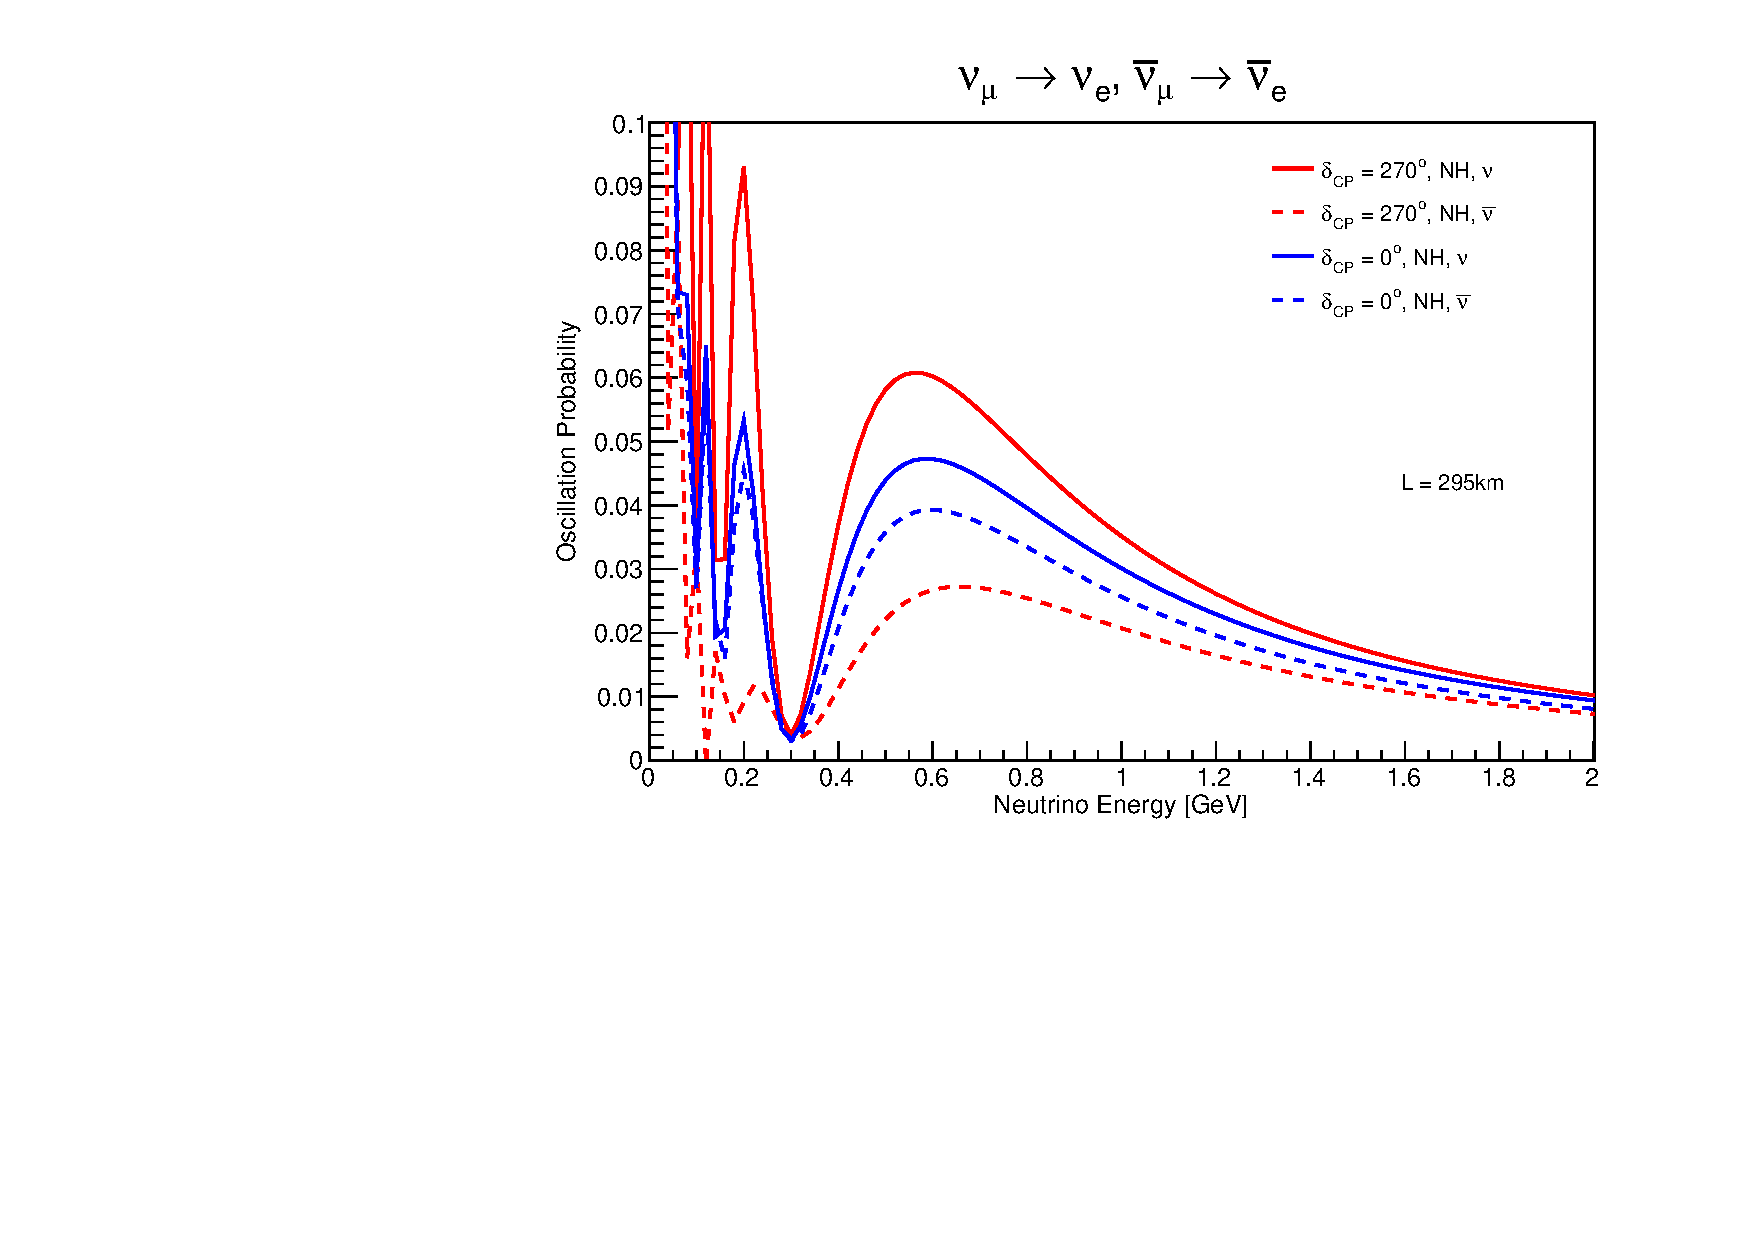
\includegraphics[width=7.5cm]{prob_t2k_compare.pdf} 
 	\caption*{}{(a)}
 \endminipage
 \hfill
\quad
 \minipage{0.485\textwidth}
 \centering
 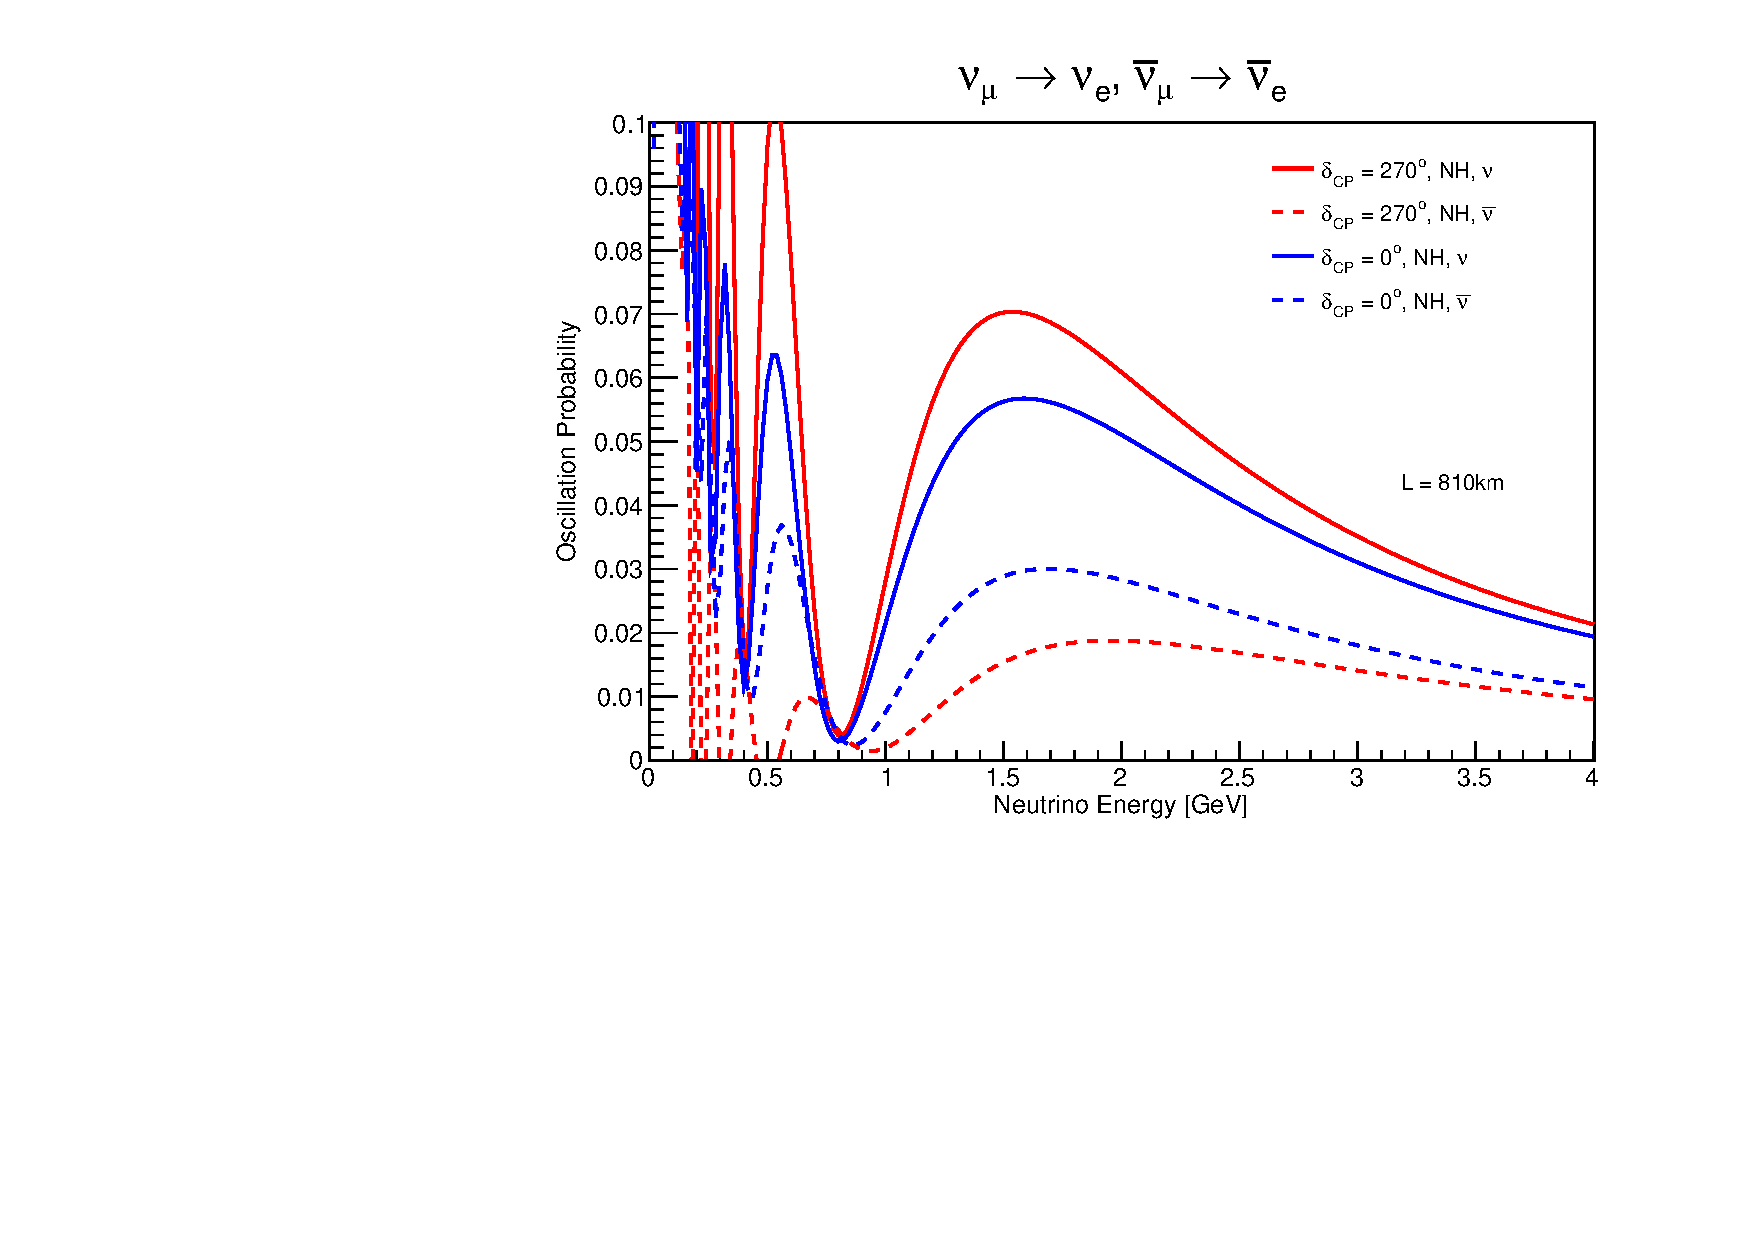
\includegraphics[width=7.5cm]{prob_nova_compare.pdf}
 \caption*{}{(b)}
 \endminipage
  \caption{{\label{fig1}} Transition probabilities $P(\nu_\mu \rightarrow \nu_e)$ and $P(\bar{\nu}_\mu \rightarrow \bar{\nu}_e)$ as a function of neutrino energy for T2K baseline $L=295$ km (a) and NO$\nu$A baseline $L=810$ km (b).}
 \hfill
 \end{figure}
 

%%%%%%%%%%%%%%%%%%%%%%%%%%%%%%%%%%%
\section{\Mr{T2K(-II) and NO$\nu$A experiments}} \label{sec:t2knova}
%%%%%%%%%%%%%%%%%%%%%%%%%%%%%%%%%%%
At present, T2K and NOvA are two leading accelerator-based long baseline neutrino experiment in the world. We briefly describe these two experiments and inputs we use to study their combined sensitivity on CP violation search.\par

 T2K (Tokai-to-Kamioka) \cite{Itow:2001ee} is an accelerator-based long-baseline neutrino oscillation experiment placed in Japan with three main complexes:  (i) the J-PARC accelerator, (ii) the near detector suite placed 280 m from the neutrino production target, and (iii) the far detector, Super-Kamiokande, situated 295 km away from target. The J-PARC, one of the most intense proton beam in the world, is used to produce a nearly pure $\bar{\nu}_{\mu}$ source. The near detector suite is designed to characterize the unoscillated neutrino beam while the far detector is used to observe the oscillation patterns. The primary goal of T2K is to observe oscillation from muon neutrinos to electron neutrinos, which has been achieved in 2013. With relatively large value of mixing angle $\theta_{13}$, the physics potential of T2K is revisited and CP violation search is placed as the central target. For the latest results ~\cite{Cao:201805}, based on a total exposure of $2.23\times 10^{21}$ POT, consisting of $1.47\times10^{21}$ POT in $\nu$-mode and $0.76\times10^{21}$ POT in $\bar{\nu}$-mode, T2K firstly reports that CP conserving value (0 and $\pi$) of $\delta_{CP}$ is out of the 2$\sigma$ C.L. range of the measurement for both normal and inverted mass hierarchies.  By the year 2021, with a fully approved exposure of $7.8 \times 10^{21}$ POT collected, T2K will have sensitivity to the CP-violating phase $\delta_{CP}$ at $90\%$ C.L. or higher over a significant range \cite{Abe:2014tzr}. To intensively explore CP violation in the lepton sector, T2K-II, extension of T2K operation up to 2026, is proposed to collect $20\times 10^{21}$ POT~\cite{Abe:2016tez}. This amount of data in combination with expected improvement in the neutrino beamline and neutrino oscillation analysis allows T2K to have 3$\sigma$ or higher significant sensitivity to CP violation. Also the oscillation parameters $\theta_{23}$ and $\Delta m^2_{31}$ can be measured at the unprecedented level.  \par
\textbf{Rescaling T2K flux}\par 
T2K flux in GLoBES which is corresponding to 2.0 degree off-axis is out of date. The new flux (50MeV wide bins) corresponding to actual 2.5 degree off-axis angle provided by Dr. Cao Son (KEK) is, however, different in format with default in GLoBES (100MeV wide bins). We therefore have to rebin it in order to be consistant with GLoBES. The rebin flux is in 100MeV wide bins up to 10GeV. All fluxes are normalized to $1 \times 10^{21}$ protons delivered to the T2K production target. The code used to rebin flux from root file and then store in txt file is provided in \textcolor{red}{rebinflux.cxx}. \par 

  \begin{figure}
   \minipage{0.485\textwidth}
 	\centering
 	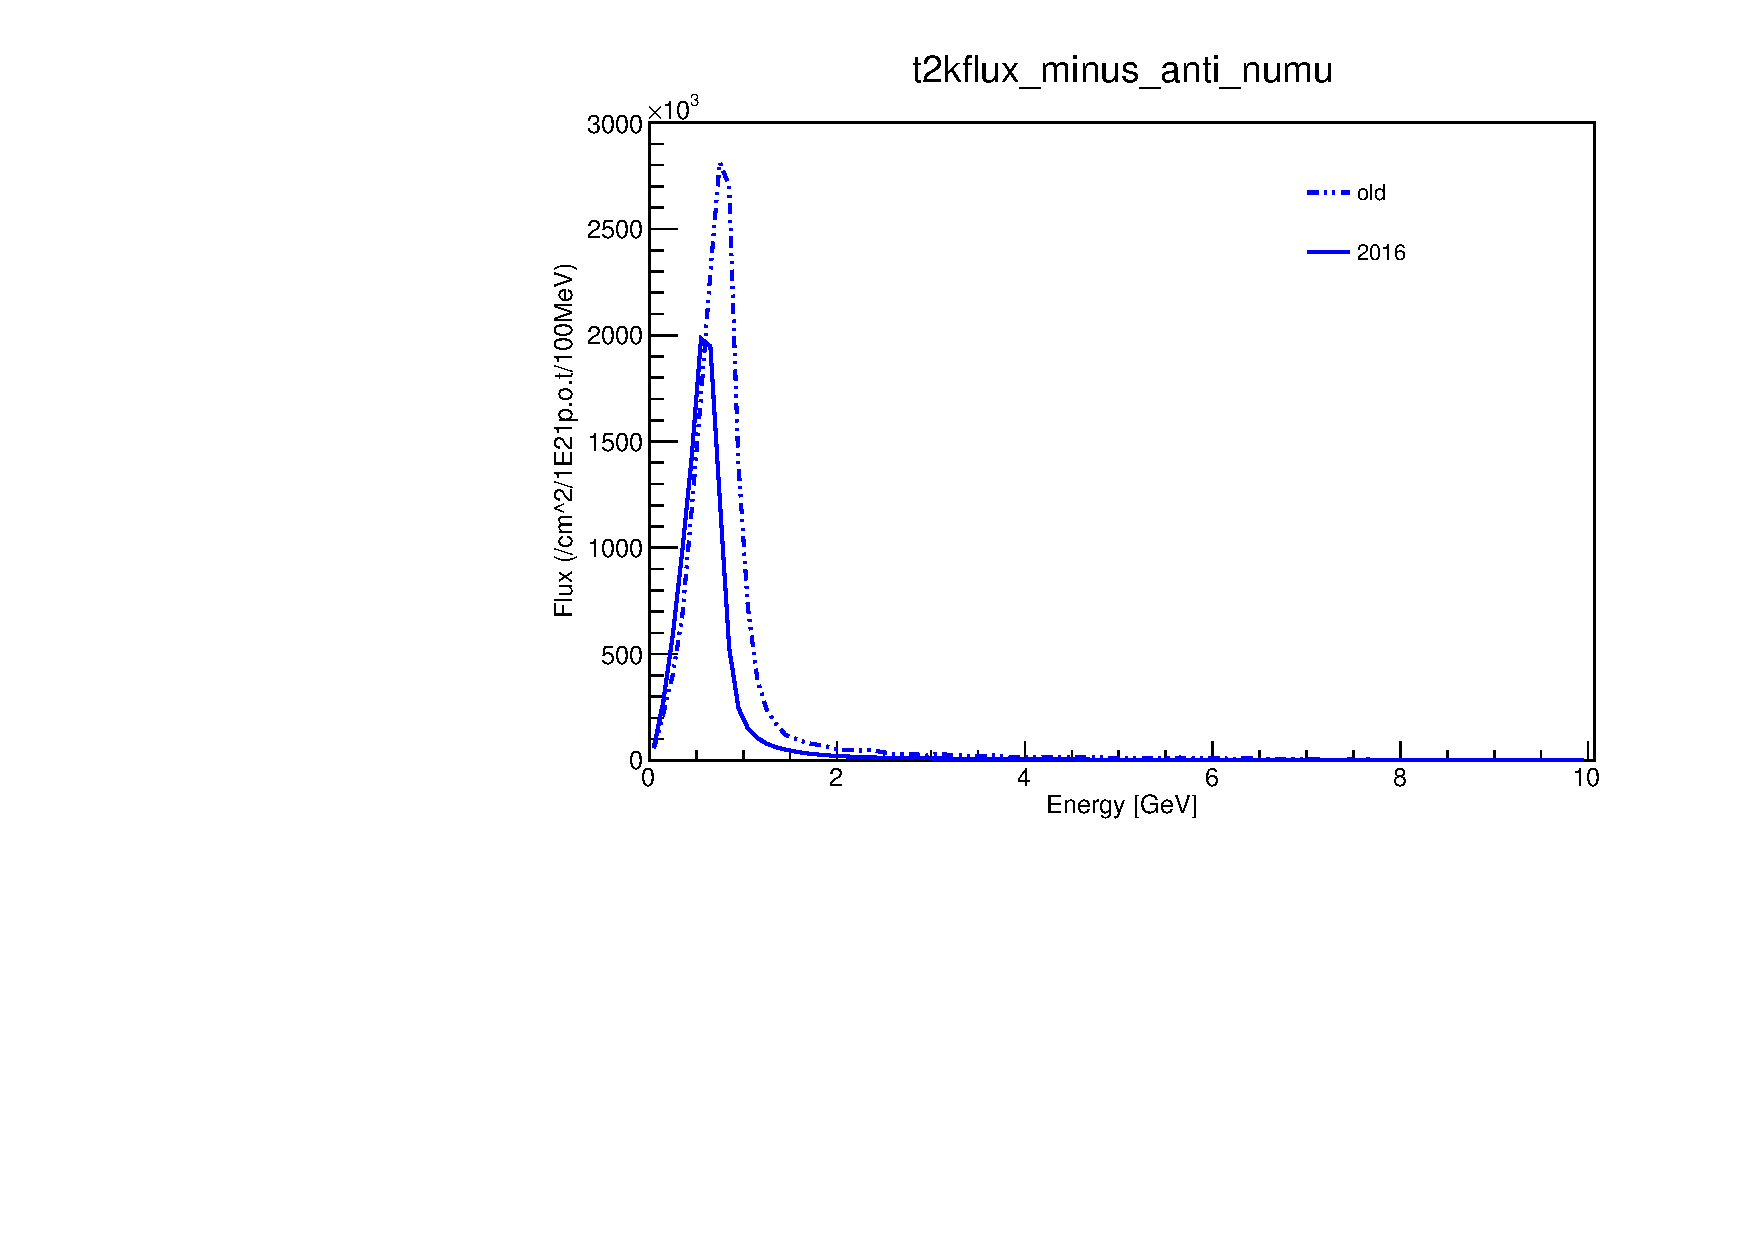
\includegraphics[width=7.5cm]{t2kflux_minus_anti_numu.pdf} 
 	\caption*{}{(a)}
 \endminipage
 \hfill
\quad
 \minipage{0.485\textwidth}
 \centering
 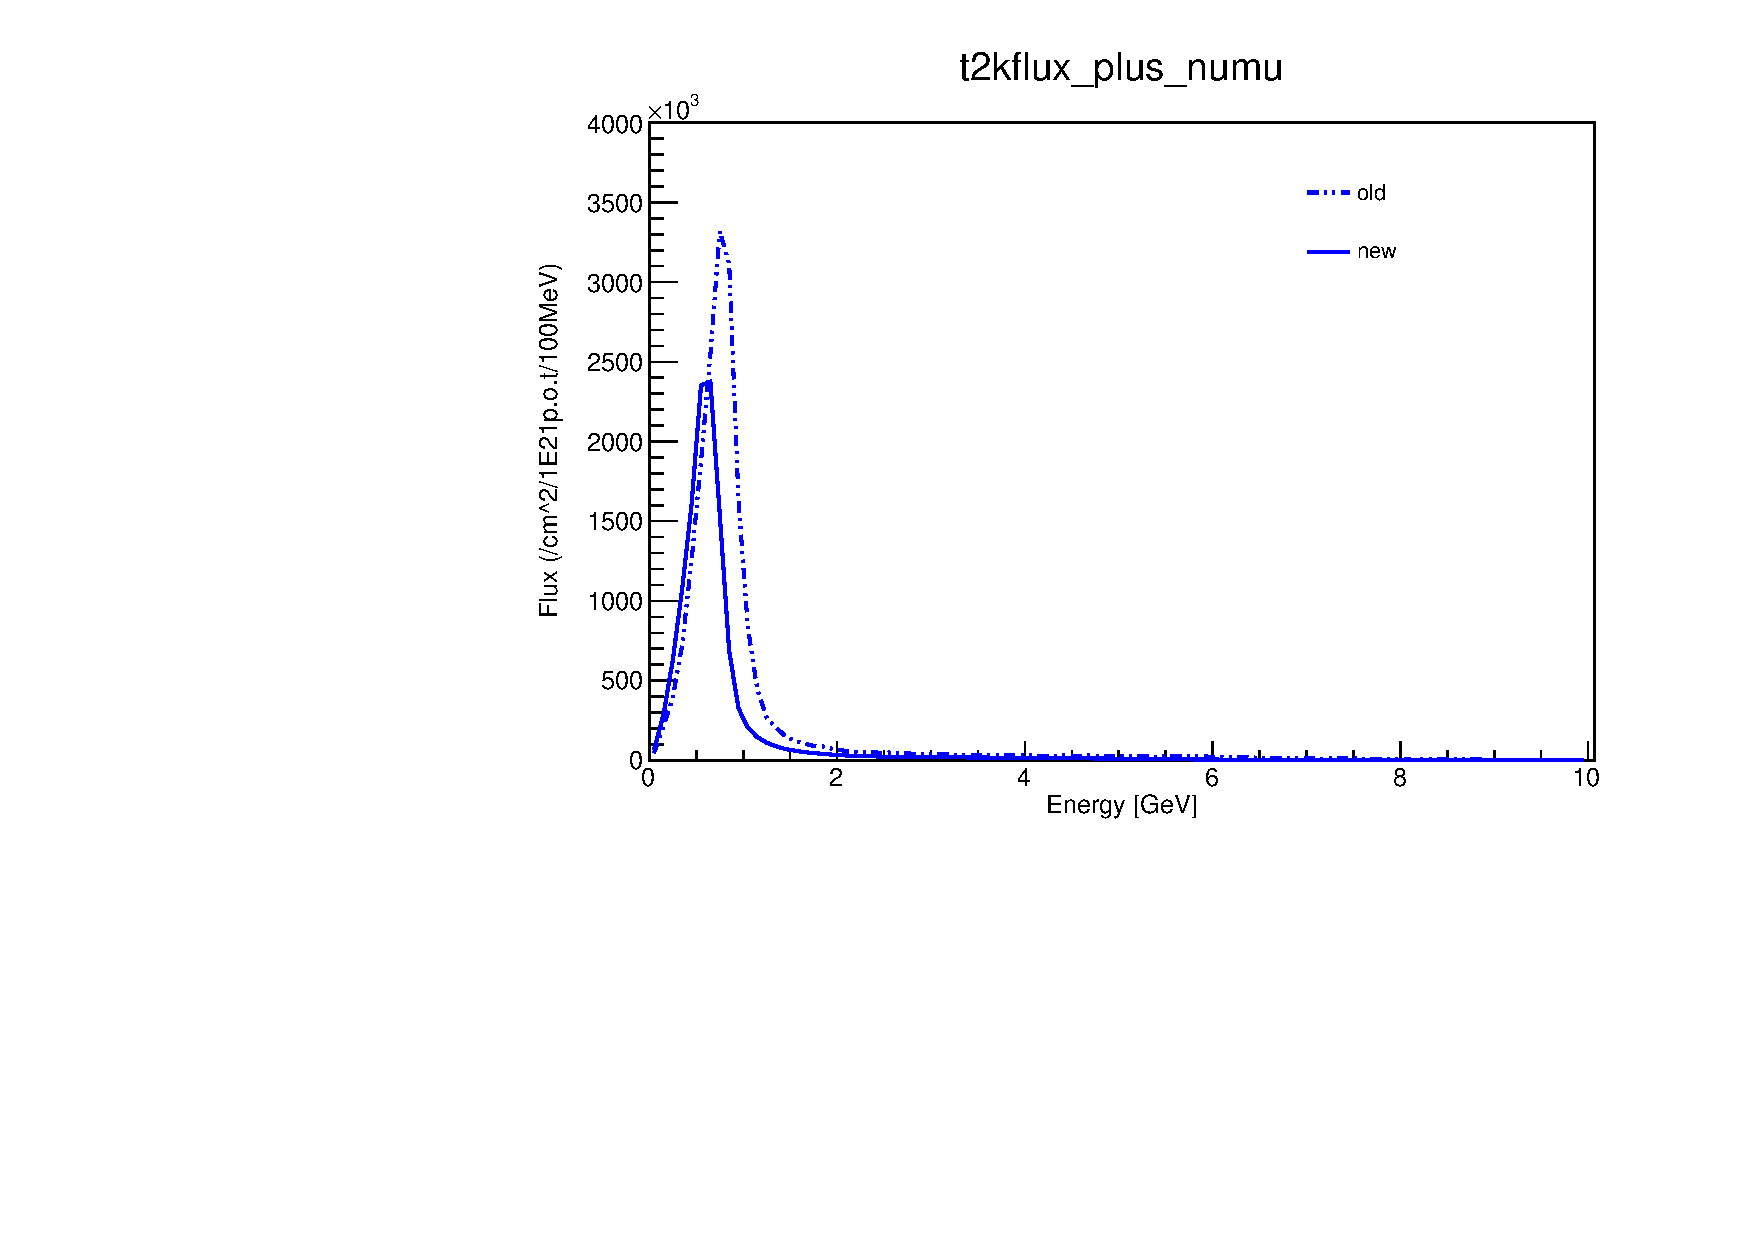
\includegraphics[width=7.5cm]{t2kflux_plus_numu.pdf}
 \caption*{}{(b)}
 \endminipage
  \caption{{\label{rebinflux}} Rebin flux compared with default in GLoBES for muon anti-neutrino beam (a) and muon neutrino beam (b).}
 \hfill
 \end{figure}


In this paper, we use GLoBES software package \cite{Huber:2002mx}  to study the physics potential of long-baseline neutrino experiments. For the inputs of T2K configuration in GloBES, we follow closely the information in the paper \cite{Abe:2016tez}. The neutrino fluxes for both neutrino-mode and antineutrino-mode operations are updated with the latest fluxes released by T2K collaboration. The full statistics of T2K-II is equivalent to 30$\times 10^{21}$ POT, which reflects the T2K-II prospect in improving the analysis with a factor of 50$\%$. The efficiencies for detecting $\nu_{e}$ and $\overline{\nu}_e$ signals are set to be $66.3\%$ and $69.7\%$ respectively while the efficiencies for detecting $\nu_{\mu}$ and $\overline{\nu}_{\mu}$ signals are 72.6$\%$ and 80.2$\%$, respectively. The event rates for T2K far detector reconstructed from GLoBES with our T2K-II setup for the cases of true $\delta_{CP} = 0,\ -\pi/2,\ +\pi/2$ are shown in the Table \ref{tab:t2knue} for $\overset{\brabar}{\nu}_{e}$ appearance samples and Table \ref{tab:t2knumu} for $\overset{\brabar}{\nu}_{\mu}$ disappearance samples. The  value here is consistent with  \cite{Abe:2016tez} at acceptable level. %Output values of the channels beam CC $\bar{\nu}_\mu$ for $\nu$-mode, beam CC $\nu_\mu$ for $\bar{\nu}$-mode in Table \ref{tab:t2knumu} are zero because these channels have not been implemented in GLoBES yet. The effect is expected to be small and we will improve this in the future.
%http://ifirse.icise.vn/nugroup/dokuwiki/doku.php?id=globes&s[]=globes

\begin{center}
\captionof{table}{The $\nu_e$ and $\bar{\nu}_e$ event samples predicted to collect in T2K-II far detector with $30 \times 10^{21}$  POT, sharing same amount for neutrino-mode and antineutrino-mode operations, at three different values of  $\delta_{CP} = -\pi/2$, $0$, $+\pi/2$. The event rates are consistent with result shown in \cite{Abe:2016tez}.}\label{tab:t2knue}
\begin{tabular}{|c| c| c| c| c| c| c| c|}
\hline
 &$\delta_{CP}$ &  Total & Signal & Signal  &  Beam CC   & Beam CC  & NC \\ 
 & &        & $\nu_\mu \rightarrow \nu_e$&$\bar{\nu}_\mu \rightarrow \bar{\nu}_e$ &   $\nu_e + \bar{\nu}_e$ &  $\nu_\mu + \bar{\nu}_\mu$ &  \\
 \hline  
\multirow{3}{*}{ $\nu$-mode $\nu_e$ sample}& $-\pi/2$ &  558.8 & 448.6 & 2.8 & 73.3 & 1.8 & 32.3 \\

 & 	0	 & 	466.3 & 354.9 	& 4.0		& 73.3	& 1.8		& 32.3\\ 
 
 & $+\pi/2$ & 370.9 & 258.6	& 4.9		& 73.3	& 1.8		& 32.3\\ 
 \hline
 
 \multirow{3}{*}{ $\overline{\nu}$-mode $\overline{\nu}_e$ sample}& $-\pi/2$ & 115.8  & 19.8 & 52.3 & 29.2 & 0.4 & 14.1 \\

 & 	0	 & 134.6	 & 16.2 	& 74.7		& 29.2	& 0.4		&14.1\\ 
 
 & $+\pi/2$ & 149.3	 & 11.8	& 93.8		& 29.2	& 0.4		& 14.1\\ 
 \hline
\end{tabular} 
\end{center}

\vspace{0.5cm}
\begin{center} 
\captionof{table}{The $\nu_\mu$ and $\bar{\nu}_\mu$ event samples predicted to collect in T2K-II far detector with $30 \times 10^{21}$ POT, sharing same amount of neutrino-mode and antineutrino-mode operations at three values of  $\delta_{CP} = -\pi/2$, $0$, $+\pi/2$. The event rates are consistent with result shown in \cite{Abe:2016tez}.}\label{tab:t2knumu}
\begin{tabular}{|c| c| c| c| c| c| c| c|}
\hline
  & $\delta_{CP}$& Total & Beam CC  &  Beam CC   & Beam CC & $\nu_\mu \rightarrow \nu_e$ +&   NC \\ 
  &    &    & $\nu_\mu $ &   $ \bar{\nu}_\mu$ &  $\nu_e + \bar{\nu}_e$ & $\bar{\nu}_\mu \rightarrow \bar{\nu}_e$ &  \\
  \hline  
  
  \multirow{3}{*}{ $\nu$-mode $\nu_{\mu}$ sample}& $-\pi/2$ &  2735.3 & 2393.3 & 158.2 & 1.6 & 7.2 & 175.0  \\

 & 	0	 & 2737.0	 &  2392.4	& 157.8		& 1.6 & 10.2 & 175.0\\ 
 
 & $+\pi/2$ & 2740.7	 &  2393.3	& 158.2		& 1.6 & 12.6 & 175.0\\ 
 \hline

  \multirow{3}{*}{ $\bar{\nu}$-mode $\overline{\nu}_{\mu}$ sample}& $-\pi/2$ &  1283.5 & 507.8 & 707.9 & 0.6 & 1.0 & 66.2  \\

 & 	0	 & 1280.5	 & 506.8 	& 706.1		& 0.6 & 0.8 & 66.2\\ 
 
 & $+\pi/2$ & 1283.1	 & 507.8	& 707.9		& 0.6 & 0.6 & 66.2\\ 
 \hline

\end{tabular} 
\end{center}

\noindent  In addition, systematic uncertainties of all T2K-II signal samples are anticipated to go down to $4\%$ compared with $5.5\% - 6.8\%$ of current level. This can be achieved by reducing errors from neutrino fluxes, neutrino interaction models and detector model uncertainties. 

 %%TOO LONG FOR T2K experiment description
 %%We care about input we use for our analysis, not their detail.
 %%also highlight their latest result and improvement can be include in the future 

%%%%%%%%%%%%%
%%%%This is to describe NOvA
%%%%%%%%%%%%%
NOvA (NuMI Off-axis $\nu_e$ Appearance) experiment~\cite{Ayres:2004js} is an accelerator-based long-baseline neutrino experiment placed in United State. NOvA uses the intense and nearly pure $\overset{\brabar}{\nu}_{\mu}$ beam from NuMI (Neutrino at Main Injector), Fermilab  and studies oscillations with two functionally identical detectors: near detector (0.3 kton) situated underground at Fermilab, Illinois and far detector (14 kton) installed on the surface in Ash River, Minesota, 810 km away from the neutrino production target. The detectors, are placed at an offset angle of 14 mrad from the average neutrino beam line in order to achieve a narrow neutrino spectrum with peak at 2 GeV and suppress the neutral current $\pi^0$ background. This configuration is optimized for observing $\nu_e$ signal. With 810 km baseline, the matter effect can change $\nu_{\mu}\rightarrow \nu_e$ appearance rate up to $\pm 30\%$. In 2017, with an equivalent exposure of $6.05\times 10^{20}$ POT, 33 $\nu_e$ candidate was observed, clearly excess from $8.2\pm 0.8$ background expected from MC. One of the major improvement in NOvA oscillation analysis is adopting machine learning algorithm, so-called Convolutional Visual Network~\cite{Aurisano:2016jvx} for the event-by-event classification of $\nu_e$ and $\overline{\nu}_e$. The gain from this new selection is equivalent to 30$\%$ effectively statistic increase. For the NOvA inputs, $61.0\%$ and $71.5\%$ signal efficiencies are used for selecting $\nu_e$ and $\overline{\nu}_e$ appearance samples, respectively. For the disappearance channels, the signal efficiencies for $\nu_{\mu}$ and $\overline{\nu}_{\mu}$ samples are  32.0$\%$ and 38.0$\%$, respectively. These number are based on the papers \cite{NOvA:2018gge} and \cite{sanchez_mayly_2018_1286758}. With an proposed operation up to the year 2024, NOvA is expected to accumulate a total exposure of $72 \times 10^{20}$ POT including $36\times 10^{20}$ in $\nu-$ mode operation and same amount for the $\bar{\nu}-$mode operation. The event rates for complete statistics of NOvA are shown in the Table \ref{tab:novanue}. In the NOvA analysis, the background from cosmic ray in the considering signal samples is significant due to the fact that the far detector is on the Earth surface. Since it is not easy to implement the cosmic ray flux in GloBES, this background is manually added into the $\nu_{\mu}$ beam neutral-current (NC) channel. The systematic uncertainty by the end of NO$\nu$A operation is assumed to be $5\%$ in GLoBES as it is provided. 


\begin{center}
\captionof{table}{The $\nu_e$ and $\bar{\nu}_e$ event rates of full statistics of NOvA operation up to 2024 with $36\times 10^{20}$ in $\nu-$ mode and $36\times 10^{20}$ in $\bar{\nu}-$mode. The rates are calculated at  at three values of  $\delta_{CP} = -\pi/2$, $0$, $+\pi/2$.}\label{tab:novanue}
\begin{tabular}{|c| c| c| c| c| c| c|}
\hline
& $\delta_{CP}$ & Total & Signal & $\nu_\mu$ beam CC   & $\nu_\mu$ beam NC  & $\nu_e$ beam \\ 
 \hline  
\multirow{3}{*}{$\nu$-mode}  &$-\pi/2$& 266.1 & 192.4 & 5.7 & 39.5 & 28.5 \\
 \multirow{3}{*}{$\nu_e$ sample}   & $0$ & 239.4 & 165.7 & 5.7 & 39.5 & 28.5 \\ 
&$+\pi/2$&  195.6 & 121.9 & 5.7 & 39.5 & 28.5 \\

\hline 
\multirow{3}{*}{$\bar{\nu}$-mode }&$-\pi/2$&  63 & 33.8 & 2.1 & 13  & 14.1 \\
\multirow{3}{*}{ $\bar{\nu}_e$ sample}&0 & 78.9 & 49.7 & 2.1 & 13 & 14.1 \\ 
& $+\pi/2$& 87.5 & 58.3 & 2.1 & 13  & 14.1  \\

\hline 
\end{tabular} 
\end{center}

\begin{center}
\captionof{table}{The $\nu_\mu$ and $\bar{\nu}_\mu$ event rates of NOvA with $36\times 10^{20}$ in $\nu-$ mode and $36\times 10^{20}$ in $\bar{\nu}-$mode. The rates are calculated at  at three values of  $\delta_{CP} = -\pi/2$, $0$, $+\pi/2$.}\label{tab:novanumu}
\begin{tabular}{|c| c| c| c| c| c|}
\hline
& $\delta_{CP}$ & Total & Signal & $\nu_\mu$ beam NC \\ 
 \hline  
  \multirow{3}{*}{ $\nu$-mode $\nu_\mu$ sample} & $-\pi/2$ & 546.3 & 512.5 & 33.8 \\
  &$0$ & 541.9 & 508.1 & 33.8 \\ 
  &$+\pi/2$ & 546.3 & 512.5 & 33.8 \\ 

\hline 
\multirow{3}{*}{ $\bar{\nu}$-mode $\bar{\nu}_\mu$ sample} &$-\pi/2$ & 276.9 & 271.3 & 5.6  \\
  &$0$ & 275 & 269.4 & 5.6  \\ 
    &$+\pi/2$ & 276.9 & 271.3 & 5.6  \\ 
\hline 
\end{tabular} 
\end{center}
%%%%%%%%%%%%%%%%%%%%%%%%%%%%%%%%%%%
\subsection{Constraint on $\theta_{13}$ from reactor}
%%%%%%%%%%%%%%%%%%%%
As mentioned before, determination of $\theta_{13}$ plays an important role in measuring $\delta_{CP}$. Current precision on $\sin^22\theta_{13}$ is $6\%$ \cite{An:2015rpe} with best fit $\sin^22\theta_{13} = 0.085$ \cite{Agashe:2014kda}. Daya Bay reactor experiment has recently approved that it can achieve $3\%$ precision on $\sin^22\theta_{13}$ by the year 2020 \cite{Cao:2016vwh}. We examine here the two above possible cases. \par 
In order to get plots as shown in Fig. \ref{theta13}, we used \textcolor{red}{Reactor2.glb}. Different constraints on $\theta_{13}$ can be obtained by changing value at \textcolor{red}{@time}.\par 
$\bullet$ @time = 60 years coressponds to $6\%$ precision on $\sin^22\theta_{13}$.\par 
$\bullet$ @time = 300 years corresponds to $3\%$ precision on $\sin^22\theta_{13}$.\par 
To make file, use \textcolor{red}{$theta13\_proj\_reactor.c$}:\par 
$\bullet$ cd to current directory.\par 
$\bullet$ run file by typing: \textcolor{blue}{$./theta13\_proj\_reactor.c$}\par 
You can change output filename in \textcolor{red}{$theta13\_proj\_reactor.c$} at\par 
\begin{center}
/* Output file */ \par 
 char MYFILE[]="$theta13\_proj\_reactor.dat$";
\end{center}\par 
To make plot, use \textcolor{red}{$plot\_theta13\_proj\_reactor.C$}\par 
To make graph containing two plots, first run \textcolor{red}{$theta13\_proj\_reactor.c$} with \textcolor{red}{@time = 60} and output file \textcolor{red}{$theta13\_proj\_reactor\_current.dat$} for $6\%$ precision. Then run \textcolor{red}{$theta13\_proj\_reactor.c$} with \textcolor{red}{@time = 300} and output file \textcolor{red}{$theta13\_proj\_reactor.dat$} for $3\%$ precision.\par 
The code to get simultanousely two plots in the same graph is provided in \par 
 \textcolor{red}{$plot\_theta13\_proj\_reactor.C$}\par
     \begin{figure}
 	\centering
 	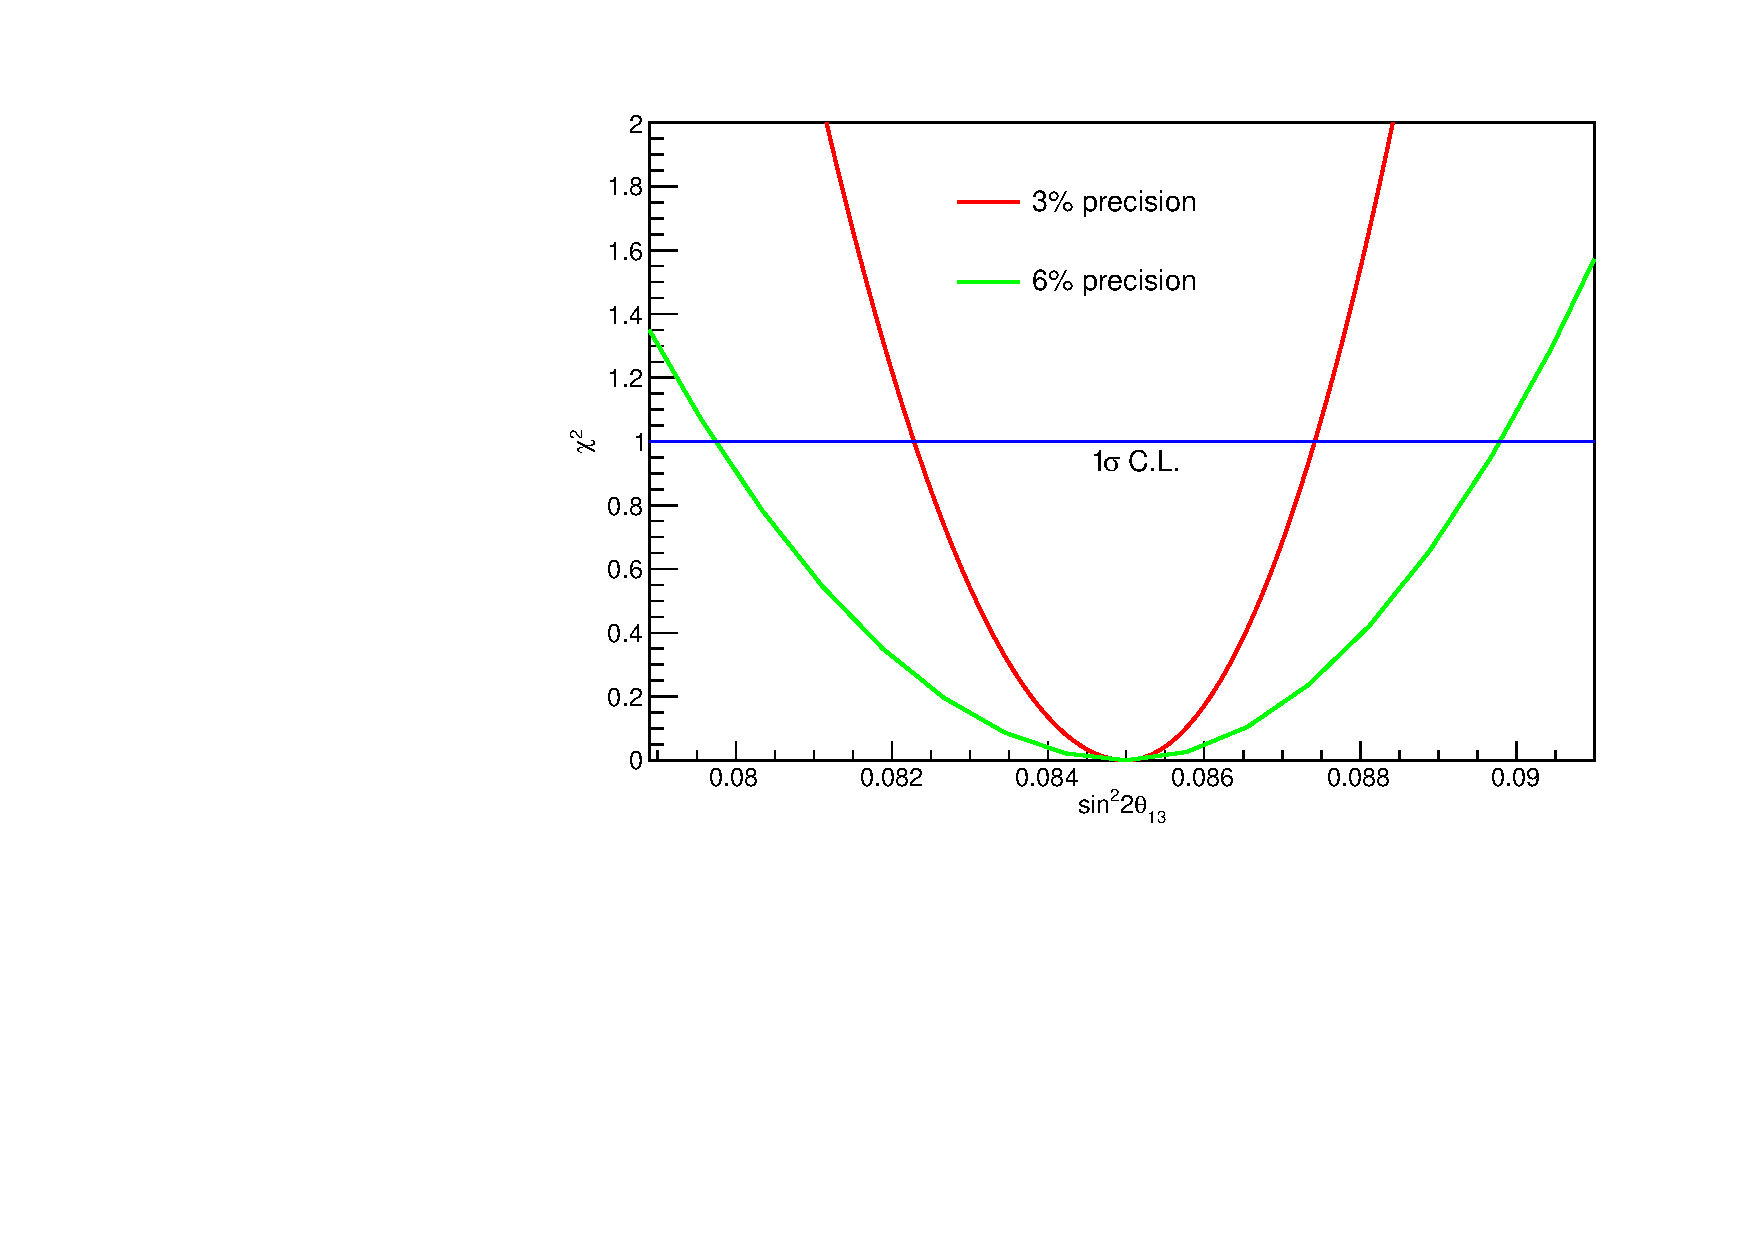
\includegraphics[scale=0.5]{theta13_precision} 
 	\caption{\label{theta13} Precision of $\theta_{13}$  from reactor. The green line corresponds to 6\% precision and the red line corresponds to 3\% precision of the current best fit value of $\sin^{2}2\theta_{13}$.} 
 \end{figure}

%%%%%%%%%%%%%%%%%%%%
%\subsection{T2K-II event rates}
%%%%%%%%%%%%%%%%%%%%
%%%%%%%%%%%%%%%%%%%%
%\subsection{NO$\nu$A event classification}
%%%%%%%%%%%%%%%%%%%%
%%%%%%%%%%%%%%%%%%%%%%%%%%%%%%%%%%%
\section{\Mr{Sensitivity to CP-violation}}\label{sec:results}
%%%%%%%%%%%%%%%%%%%%%%%%%%%%%%%%%%%

At present landscape, the value of $\delta_{CP}$ is known with marginal significant. Thus we explore the sensitivity of T2K-II and NOvA experiment on full range of this parameter. At each given value of $\delta_{CP}$, the minimal $\Delta \chi^2$ to exclude $\delta_{CP} = 0$ and $\delta_{CP} = \pm 180^{\circ}$ are calculated. These values are then plotted as a function of true $\delta_{CP}$ in the meaning to exclude $\sin\delta_{CP} = 0$. For all calculations shown below, we assume that the neutrino mass hierarchy would be known by the end of T2K-II and NOvA operations and to be normal. In the future we will explore for the case in which the neutrino mass hierarchy is unknown. Fig.~\ref{fig:sent2knova}(a) shows that T2K-II and NOvA respectively can achieve 3$\sigma$ C.L. and 2$\sigma$ C.L. to exclude CP-conserving values with current precision of mixing angle $\theta_{13}$ from reactor-based experiments, that agree with their expectations in \cite{Abe:2016tez} and \cite{sanchez_mayly_2018_1286758}. Also the figure shows that the sensitivity to CP violation is increased when the ultimate constraint on $\theta_{13}$ from reactor-based experiments is taken into account. Particularly, when $\theta_{13}$ uncertainty reduces from 6$\%$ to 3$\%$, fractional region in which the CP conserving values (0 and $\pm \pi$) can be excluded at 3$\sigma$ C.L. increases from 39.9$\%$ to 42.0$\%$ for T2K-II experiment. For NOvA, the 2$\sigma$ C.L.-excluded factional region increases from 40.8$\%$ to 41.4$\%$ when the uncertainty of $\theta_{13}$ is reduced. When the T2K-II and NOvA signal samples are combined and if the true value of $\delta_{CP}$ is close to $-\pi/2$ as indicated by T2K result, the hypothesis of CP conservation in the lepton sector can be excluded at more than 4$\sigma$ with an fractional $\delta_{CP}$ region up to 32.4$\%$ as shown in Fig.~\ref{fig:sent2knova}(b).

  \begin{figure}[H]
   \minipage{0.485\textwidth}
 	\centering
 	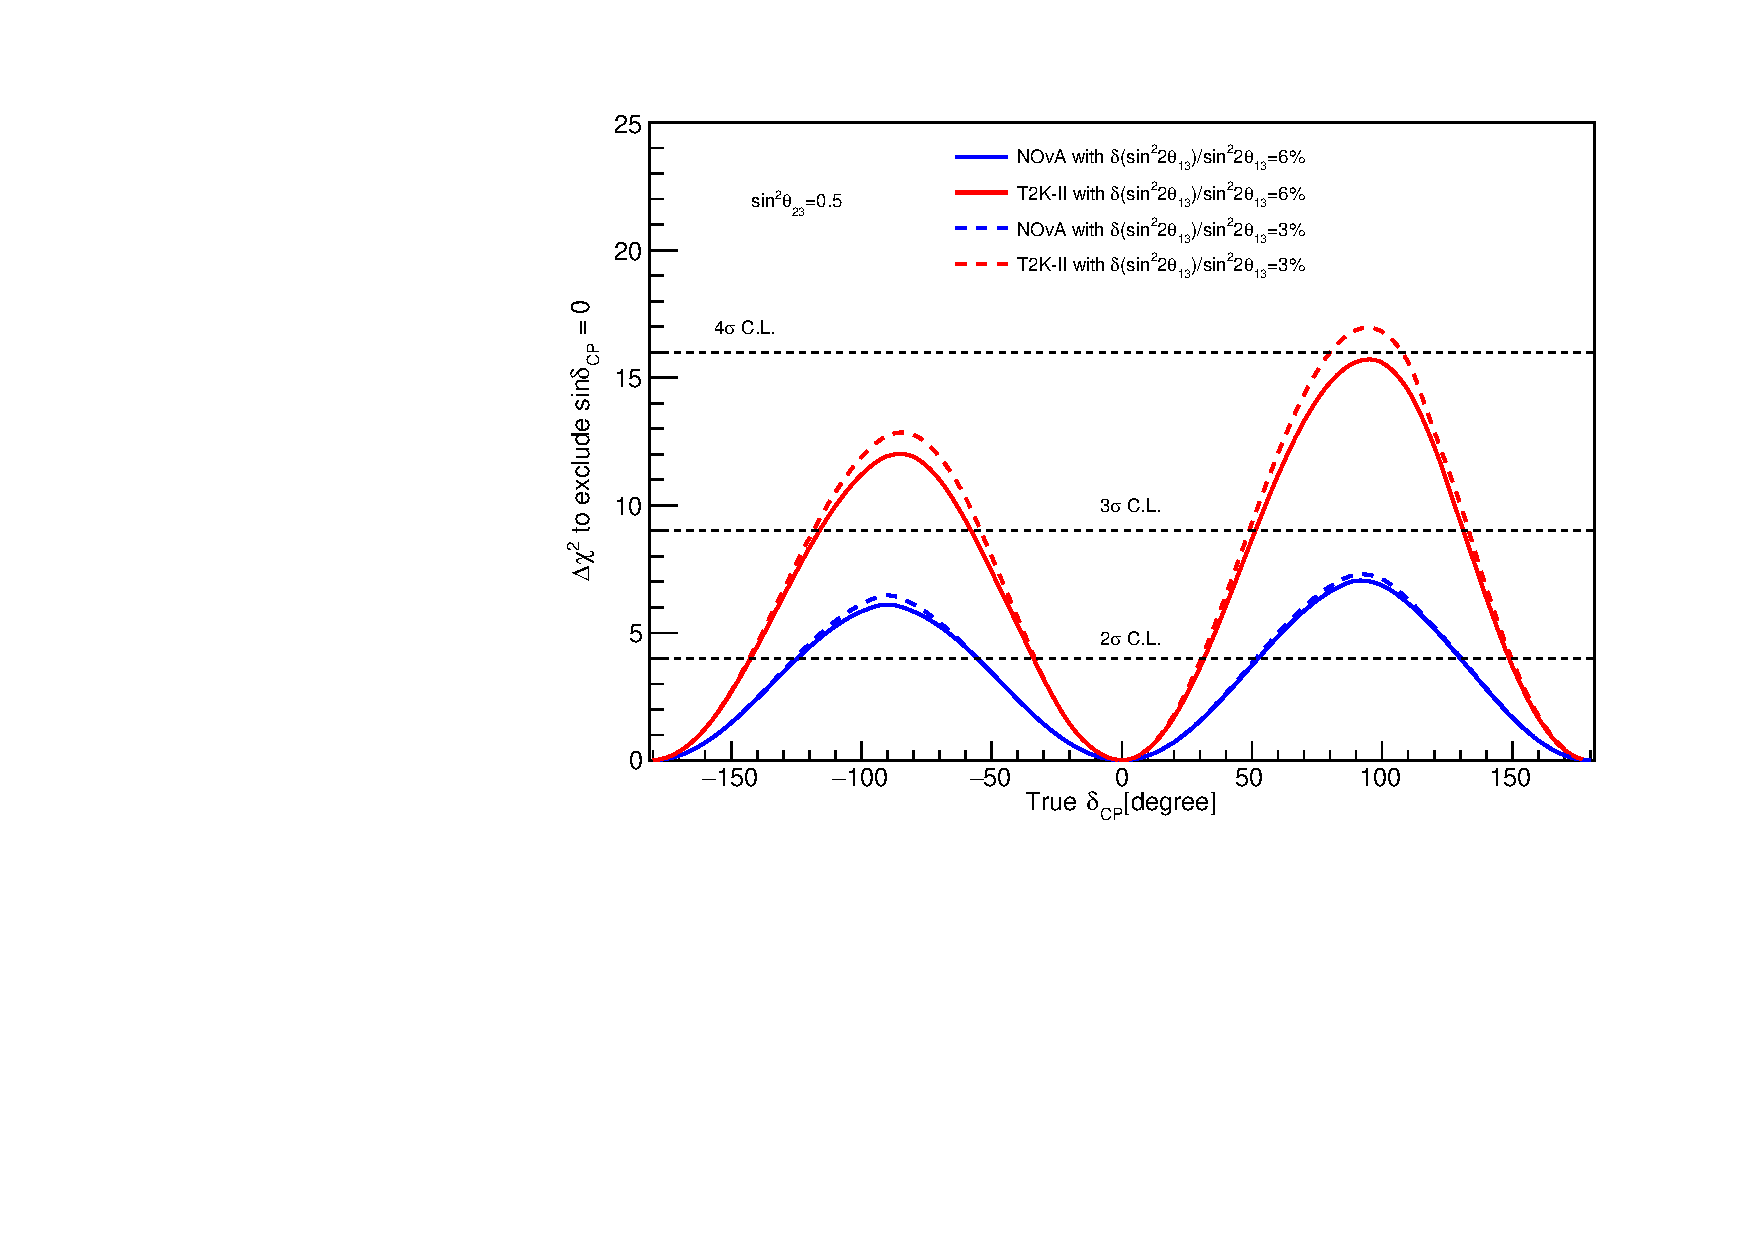
\includegraphics[width=7.5cm]{improve_th13.pdf} 
 	\caption*{}{(a)}
	\label{fig:th13eff}
 \endminipage
 \hfill
\quad
 \minipage{0.485\textwidth}
 \centering
 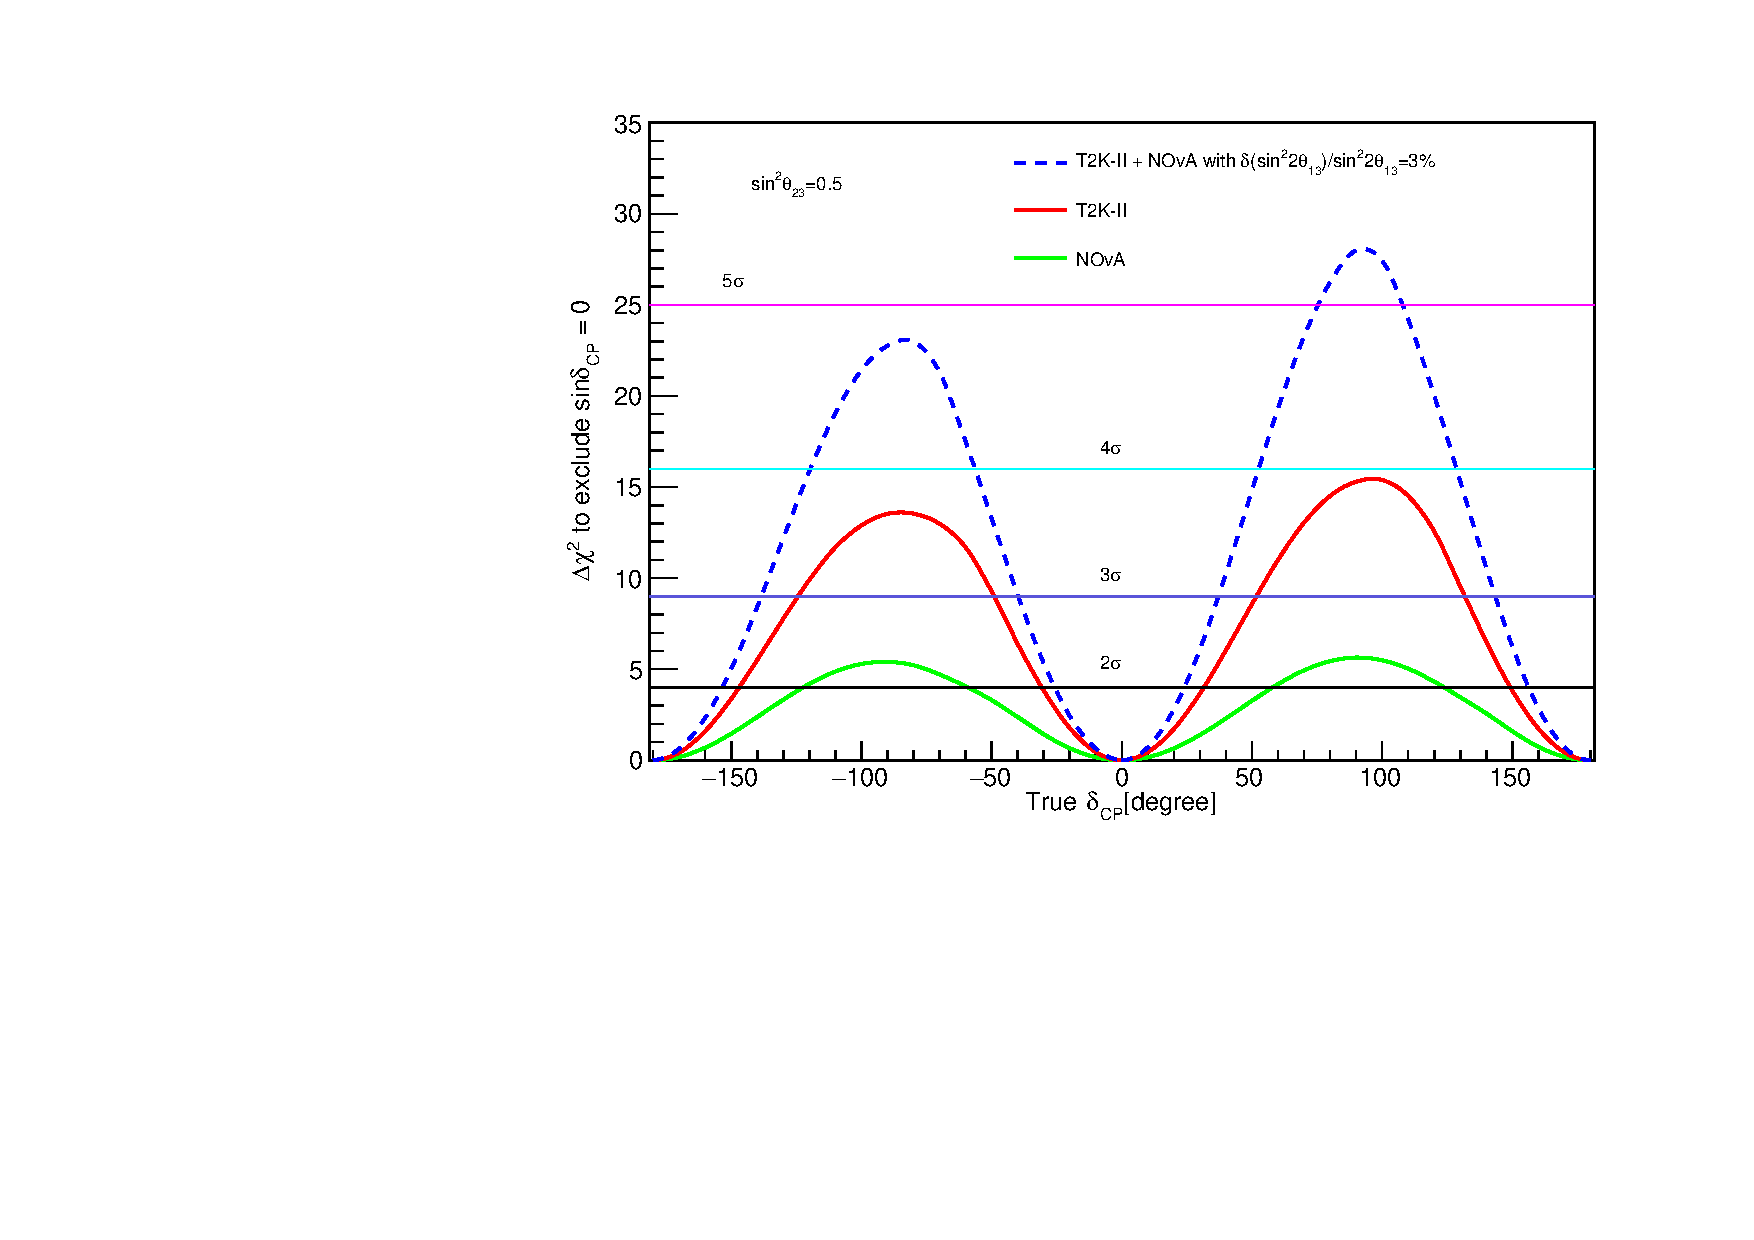
\includegraphics[width=7.5cm]{improve_nova.pdf}
 \caption*{}{(b)}
 \label{fig:combine3react}
 \endminipage
  \caption{{\label{fig:sent2knova}} (a) Sensitivity to CP-violation as a function of true $\delta_{CP}$ for T2K-II and NOvA with $6\%$ precision on $sin^2{2\theta_{13}}$ (solid red and blue lines, respectively), for T2K-II and NOvA with $3\%$ precision on $sin^2{2\theta_{13}}$ (dashed red and blue lines, respectively).\\\hspace{\textwidth}
  (b) Sensitivity to CP-violation as a function of true $\delta_{CP}$ for NOvA with $6\%$ precision on $sin^2{2\theta_{13}}$ (solid blue line), T2K-II with $6\%$ precision on $sin^2{2\theta_{13}}$ (solid red line) and T2K-II + NOvA with $3\%$ precision on $sin^2{2\theta_{13}}$ (solid black line).}
 \hfill
 \end{figure}
 
At the present, the sensitivity of CP violation in both T2K and NOvA experiments are limited predominantly by the statistics. However around 2024 to 2026 where we expect that these two experiments collect their full statistics, impact of systematics on the CP violation measurement should be considered seriously. 
In the above result, 4$\%$ and 5$\%$ uncertainties are assumed for the signal samples for T2K-II and NOvA respectively. We also check the scenario in which the uncertainties can be reduced to 2$\%$ level. The result is shown in Fig.~\ref{fig:ultisen}. Evidently improving the systematics raises significantly the level of sensitivity to CP violation. We can make discovery of CP violation at 5$\sigma$ C.L. with fractional regions of 31.2$\%$, 10.4$\%$ and 0$\%$ for 0.43, 0.5 and 0.6 of mixing angle $\sin^2\theta_{23}$, respectively.

  \begin{figure}
 	\centering
 	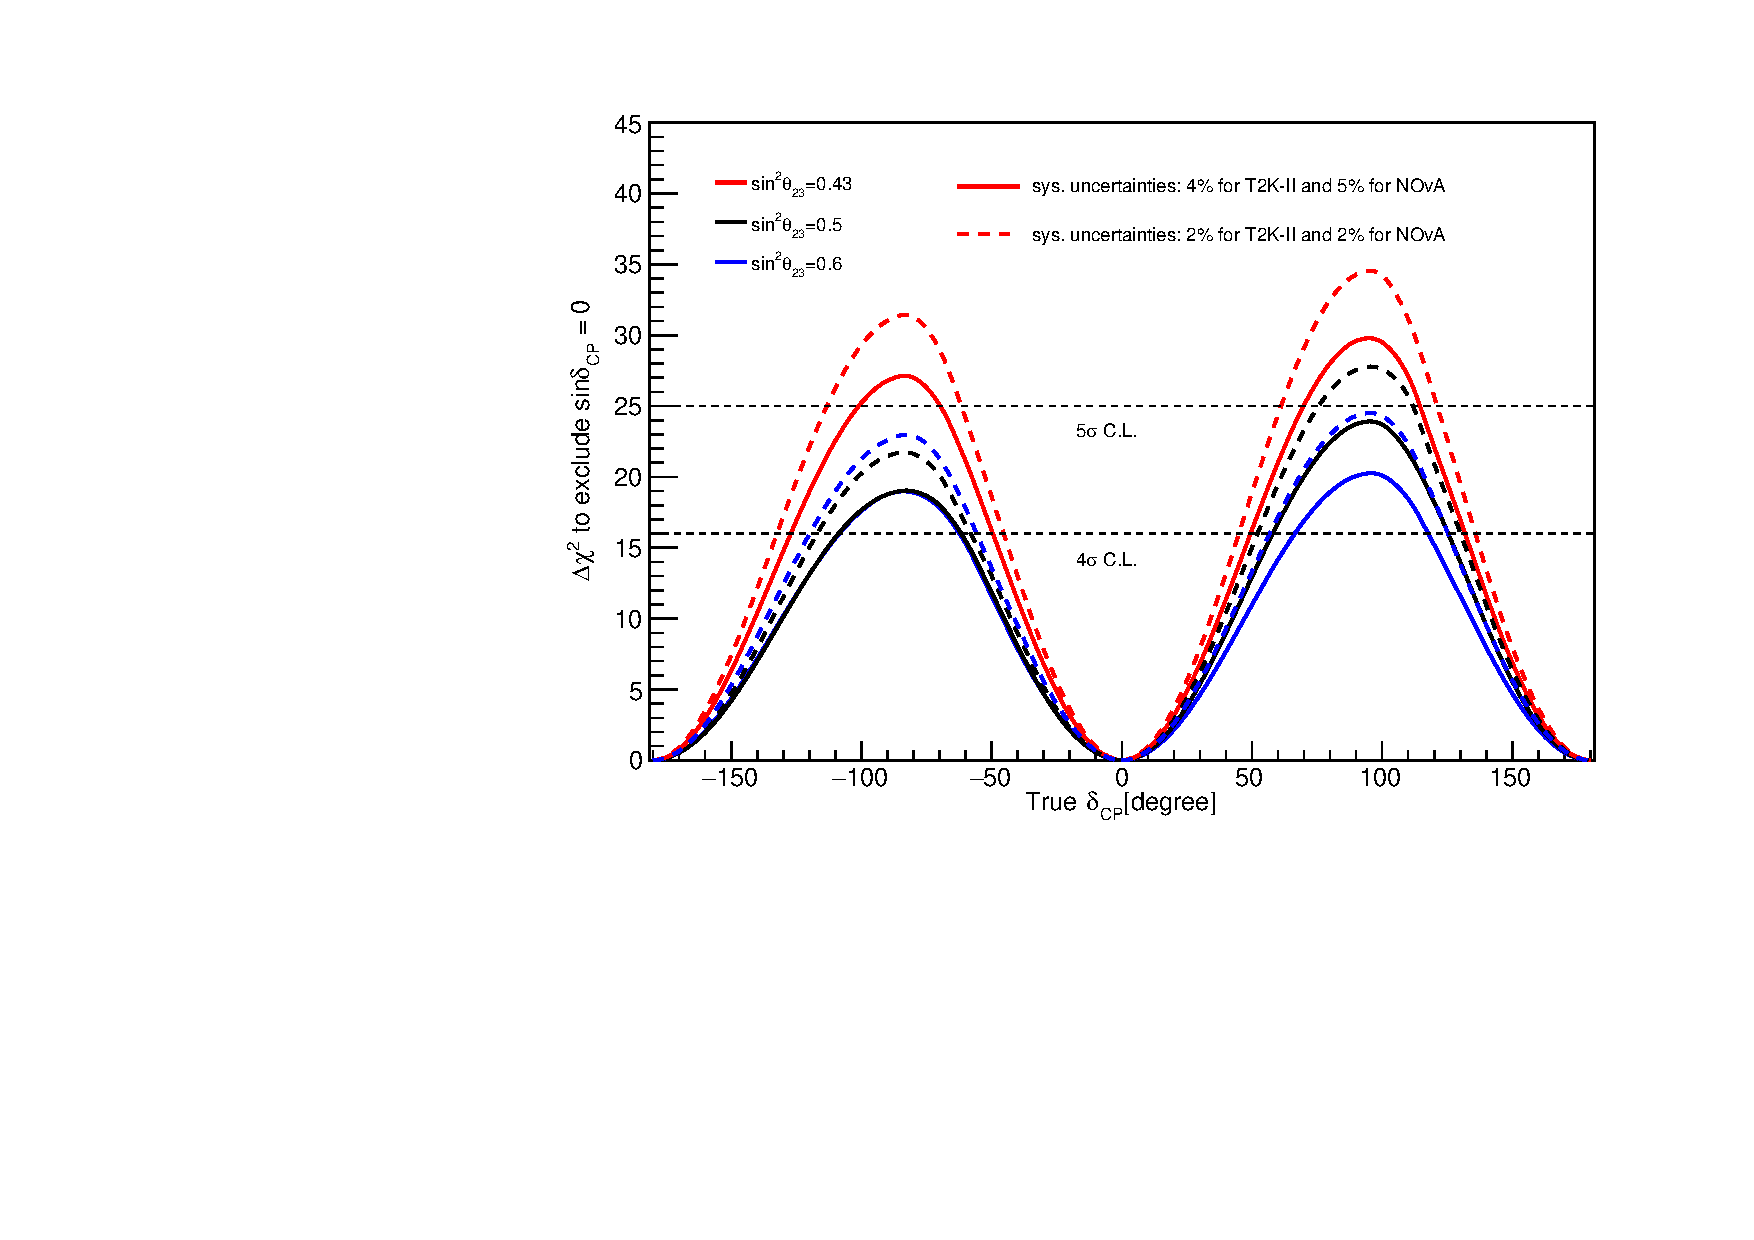
\includegraphics[scale=0.5]{improve_sys.pdf} 
 	\caption{\label{fig:ultisen} Sensitivity to CP-violation as a function of true $\delta_{CP}$ with sys. uncertainties of $4\%$ for T2K-II + $5\%$ for NOvA + ultimate reactor constraint (solid lines), and $2\%$ for T2K-II + $2\%$ for NOvA + ultimate reactor constraint (dashed lines). } 
 \end{figure}

\section{\Mr{Conclusions}}
In this paper, we have studied the sensitivity to CP-violation by combining the experiments T2K-II, which is proposed to run up to 2026, and NO$\nu$A, which can run up to 2024, with constraint from reactor-based experiments. With this combination, the CP conservation in lepton sector can be excluded at $4\sigma$ C.L. significance if the true values of $\delta_{CP}$ is around $-\pi/2$ as indicated by recent T2K measurement. The study also shows that precision measurement of mixing angle $\theta_{13}$ from the reactor-based experiments and improvements in the systematic uncertainties of measurement  are crucial for the search of CP violation in the lepton sector. We can discovery CP violation at 5$\sigma$ C.L. significance for a particular range of its value if $\theta_{13}$ precision reaches to 3$\%$ and the systematic uncertainty reduces to 2$\%$ \par 
In the near future, we will consider to improve this study for more realistic description of both T2K-II and NOvA experiments by including efficiency as function of energy, smearing matrixes between true neutrino energy and the reconstructed energy by experiments. Also adding measurements from atmospheric neutrino experiments such as Super-Kamiokande, IceCube, etc... is considered to improve our sensitivity to CP violation measurements.\par 

\bibliographystyle{unsrt}
\bibliography{reference}

\begin{thebibliography}{9}
%\cite{Cleveland:1998nv}
\bibitem{Cleveland:1998nv} 
  B.~T.~Cleveland, T.~Daily, R.~Davis, Jr., J.~R.~Distel, K.~Lande, C.~K.~Lee, P.~S.~Wildenhain and J.~Ullman,
  %``Measurement of the solar electron neutrino flux with the Homestake chlorine detector,''
  Astrophys.\ J.\  {\bf 496}, 505 (1998).
  doi:10.1086/305343
  %%CITATION = doi:10.1086/305343;%%
  %2359 citations counted in INSPIRE as of 08 May 2018

%\cite{Hirata:1988uy}
\bibitem{Hirata:1988uy} 
  K.~S.~Hirata {\it et al.} [Kamiokande-II Collaboration],
  %``Experimental Study of the Atmospheric Neutrino Flux,''
  Phys.\ Lett.\ B {\bf 205}, 416 (1988).
  doi:10.1016/0370-2693(88)91690-5
  %%CITATION = doi:10.1016/0370-2693(88)91690-5;%%
  %846 citations counted in INSPIRE as of 08 May 2018

%\cite{Pontecorvo:1957cp}
\bibitem{Pontecorvo:1957cp} 
  B.~Pontecorvo,
  %``Mesonium and anti-mesonium,''
  Sov.\ Phys.\ JETP {\bf 6}, 429 (1957)
  [Zh.\ Eksp.\ Teor.\ Fiz.\  {\bf 33}, 549 (1957)].
  %%CITATION = SPHJA,6,429;%%
  %1705 citations counted in INSPIRE as of 08 May 2018


%\cite{Maki:1962mu}
\bibitem{Maki:1962mu} 
  Z.~Maki, M.~Nakagawa and S.~Sakata,
  %``Remarks on the unified model of elementary particles,''
  Prog.\ Theor.\ Phys.\  {\bf 28}, 870 (1962).
  doi:10.1143/PTP.28.870
  %%CITATION = doi:10.1143/PTP.28.870;%%
  %3403 citations counted in INSPIRE as of 08 May 2018
  
  \bibitem{Patrignani:2016xqp}
  C.~Patrignani {\it et al.},
  %``Review of Particle Physics,''
  Chin.\ Phys.\ C {\bf 40}, no. 10, 100001 (2016).
 % doi:10.1088/1674-1137/40/10/100001
  %%CITATION = doi:10.1088/1674-1137/40/10/100001;%%
  %3180 citations counted in INSPIRE as of 29 Apr 2018


 %\cite{Abe:2014tzr}
\bibitem{Abe:2014tzr} 
  K.~Abe {\it et al.} [T2K Collaboration],
  %``Neutrino oscillation physics potential of the T2K experiment,''
  PTEP {\bf 2015}, no. 4, 043C01 (2015)
  doi:10.1093/ptep/ptv031
  [arXiv:1409.7469 [hep-ex]].
  %%CITATION = doi:10.1093/ptep/ptv031;%%
  %85 citations counted in INSPIRE as of 11 May 2018
  
%\cite{An:2013uza}
\bibitem{An:2013uza} 
  F.~P.~An {\it et al.} [Daya Bay Collaboration],
  %``Improved Measurement of Electron Antineutrino Disappearance at Daya Bay,''
  Chin.\ Phys.\ C {\bf 37}, 011001 (2013)
  doi:10.1088/1674-1137/37/1/011001
  [arXiv:1210.6327 [hep-ex]].
  %%CITATION = doi:10.1088/1674-1137/37/1/011001;%%
  %379 citations counted in INSPIRE as of 08 May 2018



%\cite{Ahn:2012nd}
\bibitem{Ahn:2012nd} 
  J.~K.~Ahn {\it et al.} [RENO Collaboration],
  %``Observation of Reactor Electron Antineutrino Disappearance in the RENO Experiment,''
  Phys.\ Rev.\ Lett.\  {\bf 108}, 191802 (2012)
  doi:10.1103/PhysRevLett.108.191802
  [arXiv:1204.0626 [hep-ex]].
  %%CITATION = doi:10.1103/PhysRevLett.108.191802;%%
  %1714 citations counted in INSPIRE as of 08 May 2018


%\cite{Abe:2012tg}
\bibitem{Abe:2012tg} 
  Y.~Abe {\it et al.} [Double Chooz Collaboration],
  %``Reactor electron antineutrino disappearance in the Double Chooz experiment,''
  Phys.\ Rev.\ D {\bf 86}, 052008 (2012)
  doi:10.1103/PhysRevD.86.052008
  [arXiv:1207.6632 [hep-ex]].
  %%CITATION = doi:10.1103/PhysRevD.86.052008;%%
  %427 citations counted in INSPIRE as of 08 May 2018
  


%\cite{Itow:2001ee}
\bibitem{Itow:2001ee} 
  Y.~Itow {\it et al.} [T2K Collaboration],
  %``The JHF-Kamioka neutrino project,''
  hep-ex/0106019.
  %%CITATION = HEP-EX/0106019;%%
  %1010 citations counted in INSPIRE as of 08 May 2018

  
  %\cite{Abe:2014tzr}
\bibitem{Abe:2014tzr} 
  K.~Abe {\it et al.} [T2K Collaboration],
  %``Neutrino oscillation physics potential of the T2K experiment,''
  PTEP {\bf 2015}, no. 4, 043C01 (2015)
  doi:10.1093/ptep/ptv031
  [arXiv:1409.7469 [hep-ex]].
  %%CITATION = doi:10.1093/ptep/ptv031;%%
  %85 citations counted in INSPIRE as of 08 May 2018
  

%\cite{Abe:2016tez}
\bibitem{Abe:2016tez} 
  K.~Abe {\it et al.} [T2K Collaboration],
  %``Sensitivity of the T2K accelerator-based neutrino experiment with an Extended run to $20\times10^{21}$ POT,''
  arXiv:1607.08004 [hep-ex].
  %%CITATION = ARXIV:1607.08004;%%
  %11 citations counted in INSPIRE as of 08 May 2018
 
 

%\cite{Ayres:2004js}
\bibitem{Ayres:2004js}
  D.~S.~Ayres {\it et al.} [NOvA Collaboration],
  ``NOvA: Proposal to Build a 30 Kiloton Off-Axis Detector to Study $\nu_{\mu} \to \nu_e$ Oscillations in the NuMI Beamline,''
  hep-ex/0503053.
  %%CITATION = HEP-EX/0503053;%%
  %677 citations counted in INSPIRE as of 08 May 2018
  

%\bibitem{nova project diappearance} \label{a18}
% T. Yang and S. Woijcicki.    
%\textit{Study of physics sensitivity of $\nu_mu$ disappearance in a totally active version of NoVA detector}. 
%Off-Axis-Note-SIM-30 (2004).

 
 
%\cite{Adamson:2017gxd}
\bibitem{Adamson:2017gxd} 
  P.~Adamson {\it et al.} [NOvA Collaboration],
  %``Constraints on Oscillation Parameters from $\nu_e$ Appearance and $\nu_\mu$ Disappearance in NOvA,''
  Phys.\ Rev.\ Lett.\  {\bf 118}, no. 23, 231801 (2017)
  doi:10.1103/PhysRevLett.118.231801
  [arXiv:1703.03328 [hep-ex]].
  %%CITATION = doi:10.1103/PhysRevLett.118.231801;%%
  %68 citations counted in INSPIRE as of 08 May 2018  



%\cite{Huber:2002mx}
\bibitem{Huber:2002mx} 
  P.~Huber, M.~Lindner and W.~Winter,
  %``Superbeams versus neutrino factories,''
  Nucl.\ Phys.\ B {\bf 645}, 3 (2002)
  doi:10.1016/S0550-3213(02)00825-8
  [hep-ph/0204352].
  %%CITATION = doi:10.1016/S0550-3213(02)00825-8;%%
  %327 citations counted in INSPIRE as of 08 May 2018
  
  %\cite{Cao:2016vwh}
\bibitem{Cao:2016vwh} 
  J.~Cao and K.~B.~Luk,
  %``An overview of the Daya Bay Reactor Neutrino Experiment,''
  Nucl.\ Phys.\ B {\bf 908}, 62 (2016)
  doi:10.1016/j.nuclphysb.2016.04.034
  [arXiv:1605.01502 [hep-ex]].
  %%CITATION = doi:10.1016/j.nuclphysb.2016.04.034;%%
  %5 citations counted in INSPIRE as of 08 May 2018
  
  %\cite{An:2015rpe}
\bibitem{An:2015rpe} 
  F.~P.~An {\it et al.} [Daya Bay Collaboration],
  %``New Measurement of Antineutrino Oscillation with the Full Detector Configuration at Daya Bay,''
  Phys.\ Rev.\ Lett.\  {\bf 115}, no. 11, 111802 (2015)
  doi:10.1103/PhysRevLett.115.111802
  [arXiv:1505.03456 [hep-ex]].
  %%CITATION = doi:10.1103/PhysRevLett.115.111802;%%
  %158 citations counted in INSPIRE as of 08 May 2018





%\cite{Agashe:2014kda}
\bibitem{Agashe:2014kda} 
  K.~A.~Olive {\it et al.} [Particle Data Group],
  %``Review of Particle Physics,''
  Chin.\ Phys.\ C {\bf 38}, 090001 (2014).
  doi:10.1088/1674-1137/38/9/090001
  %%CITATION = doi:10.1088/1674-1137/38/9/090001;%%
  %7218 citations counted in INSPIRE as of 08 May 2018



\bibitem{Sato} \label{a6}
Jiro Arafune, Masafumi Koike and Joe Sato.  
\textit{CP Violation and Matter Effect in Long Baseline Neutrino Oscillation Experiments}. 
arXiv:hep-ph/9703351v5 8 Jul 1999.

%\cite{Arafune:1997hd}
\bibitem{Arafune:1997hd} 
  J.~Arafune, M.~Koike and J.~Sato,
  %``CP violation and matter effect in long baseline neutrino oscillation experiments,''
  Phys.\ Rev.\ D {\bf 56}, 3093 (1997)
  Erratum: [Phys.\ Rev.\ D {\bf 60}, 119905 (1999)]
  doi:10.1103/PhysRevD.60.119905, 10.1103/PhysRevD.56.3093
  [hep-ph/9703351].
  %%CITATION = doi:10.1103/PhysRevD.60.119905, 10.1103/PhysRevD.56.3093;%%
  %235 citations counted in INSPIRE as of 08 May 2018

%\bibitem{Solar problems} \label{a9}
%J. N. Bahcall, W. A. Fowler, I. Iben Jr. and R. L. Sears.  
%\textit{Solar neutrino flux}. 
%Astrophys. J 137 344 (1963).

%\cite{Bahcall:1997ha}
%\bibitem{Bahcall:1997ha} 
 % J.~N.~Bahcall, W.~A.~Fowler, I.~Iben, Jr. and R.~L.~Sears,
  %``Solar neutrino flux,''
  %Astrophys.\ J.\  {\bf 137}, 344 (1963).
  %doi:10.1086/147513
  %%CITATION = doi:10.1086/147513;%%
  %96 citations counted in INSPIRE as of 08 May 2018


%\bibitem{Solar problems} \label{a10}
%R. L. Sears. 
%\textit{Helium Content and Neutrino Fluxes in Solar Models}. 
%Astrophys. J 140 477 (1964).

%\bibitem{atmospheric neutrino Super-K} \label{a13}
%Y. Fukuda et al.    
%\textit{Evidence for oscillation of atmospheric neutrinos}. 
%Phys. Rev. Lett. 81 5162-1567 (1998).


%\bibitem{solar neutrino Super-K} \label{a14}
%Y. Fukuda et al.    
%\textit{Measurements of the solar neutrino flux from Super-Kamiokande's first 300 days}. 
%Phys. Rev. Lett. 81 1158-1162 (1998).


%\cite{Fukuda:1998mi}
\bibitem{Fukuda:1998mi} 
  Y.~Fukuda {\it et al.} [Super-Kamiokande Collaboration],
  %``Evidence for oscillation of atmospheric neutrinos,''
  Phys.\ Rev.\ Lett.\  {\bf 81}, 1562 (1998)
  doi:10.1103/PhysRevLett.81.1562
  [hep-ex/9807003].
  %%CITATION = doi:10.1103/PhysRevLett.81.1562;%%
  %5467 citations counted in INSPIRE as of 08 May 2018

%\cite{Ahmad:2001an}
\bibitem{Ahmad:2001an} 
  Q.~R.~Ahmad {\it et al.} [SNO Collaboration],
  %``Measurement of the rate of $\nu_e+d \to p+p+e^-$ interactions produced by $^8B$ solar neutrinos at the Sudbury Neutrino Observatory,''
  Phys.\ Rev.\ Lett.\  {\bf 87}, 071301 (2001)
  doi:10.1103/PhysRevLett.87.071301
  [nucl-ex/0106015].
  %%CITATION = doi:10.1103/PhysRevLett.87.071301;%%
  %2508 citations counted in INSPIRE as of 08 May 2018




\bibitem{Patrignani:2016xqp} 
  C.~Patrignani {\it et al.},
  %``Review of Particle Physics,''
  {\it Chin.\ Phys.}\ C {\bf 40}, no. 10, 100001 (2016).
 % doi:10.1088/1674-1137/40/10/100001
  %%CITATION = doi:10.1088/1674-1137/40/10/100001;%%
  %3180 citations counted in INSPIRE as of 29 Apr 2018

%\cite{Abe:2013hdq}
\bibitem{Abe:2013hdq} 
  K.~Abe {\it et al.} [T2K Collaboration],
  %``Observation of Electron Neutrino Appearance in a Muon Neutrino Beam,''
  Phys.\ Rev.\ Lett.\  {\bf 112}, 061802 (2014)
  doi:10.1103/PhysRevLett.112.061802
  [arXiv:1311.4750 [hep-ex]].
  %%CITATION = doi:10.1103/PhysRevLett.112.061802;%%
  %470 citations counted in INSPIRE as of 20 May 2018


%\cite{Cao:201805}
\bibitem{Cao:201805} 
  C. V.~Son [for T2K Collaboration],
  %``Sensitivity of the T2K accelerator-based neutrino experiment with an Extended run to $20\times10^{21}$ POT,''
  arXiv:1805.05917 [hep-ex].
  %%CITATION = ARXIV:1607.08004;%%
  %11 citations counted in INSPIRE as of 08 May 2018
  
  %\cite{Aurisano:2016jvx}
\bibitem{Aurisano:2016jvx} 
  A.~Aurisano {\it et al.},
  %``A Convolutional Neural Network Neutrino Event Classifier,''
  JINST {\bf 11}, no. 09, P09001 (2016)
  doi:10.1088/1748-0221/11/09/P09001
  [arXiv:1604.01444 [hep-ex]].
  %%CITATION = doi:10.1088/1748-0221/11/09/P09001;%%
  %46 citations counted in INSPIRE as of 21 May 2018

\end{thebibliography}
 

\end{document}


\end{document}
